% Options for packages loaded elsewhere
\PassOptionsToPackage{unicode}{hyperref}
\PassOptionsToPackage{hyphens}{url}
\PassOptionsToPackage{dvipsnames,svgnames,x11names}{xcolor}
%
\documentclass[
  letterpaper,
  DIV=11,
  numbers=noendperiod]{scrartcl}

\usepackage{amsmath,amssymb}
\usepackage{iftex}
\ifPDFTeX
  \usepackage[T1]{fontenc}
  \usepackage[utf8]{inputenc}
  \usepackage{textcomp} % provide euro and other symbols
\else % if luatex or xetex
  \usepackage{unicode-math}
  \defaultfontfeatures{Scale=MatchLowercase}
  \defaultfontfeatures[\rmfamily]{Ligatures=TeX,Scale=1}
\fi
\usepackage{lmodern}
\ifPDFTeX\else  
    % xetex/luatex font selection
\fi
% Use upquote if available, for straight quotes in verbatim environments
\IfFileExists{upquote.sty}{\usepackage{upquote}}{}
\IfFileExists{microtype.sty}{% use microtype if available
  \usepackage[]{microtype}
  \UseMicrotypeSet[protrusion]{basicmath} % disable protrusion for tt fonts
}{}
\makeatletter
\@ifundefined{KOMAClassName}{% if non-KOMA class
  \IfFileExists{parskip.sty}{%
    \usepackage{parskip}
  }{% else
    \setlength{\parindent}{0pt}
    \setlength{\parskip}{6pt plus 2pt minus 1pt}}
}{% if KOMA class
  \KOMAoptions{parskip=half}}
\makeatother
\usepackage{xcolor}
\setlength{\emergencystretch}{3em} % prevent overfull lines
\setcounter{secnumdepth}{5}
% Make \paragraph and \subparagraph free-standing
\makeatletter
\ifx\paragraph\undefined\else
  \let\oldparagraph\paragraph
  \renewcommand{\paragraph}{
    \@ifstar
      \xxxParagraphStar
      \xxxParagraphNoStar
  }
  \newcommand{\xxxParagraphStar}[1]{\oldparagraph*{#1}\mbox{}}
  \newcommand{\xxxParagraphNoStar}[1]{\oldparagraph{#1}\mbox{}}
\fi
\ifx\subparagraph\undefined\else
  \let\oldsubparagraph\subparagraph
  \renewcommand{\subparagraph}{
    \@ifstar
      \xxxSubParagraphStar
      \xxxSubParagraphNoStar
  }
  \newcommand{\xxxSubParagraphStar}[1]{\oldsubparagraph*{#1}\mbox{}}
  \newcommand{\xxxSubParagraphNoStar}[1]{\oldsubparagraph{#1}\mbox{}}
\fi
\makeatother


\providecommand{\tightlist}{%
  \setlength{\itemsep}{0pt}\setlength{\parskip}{0pt}}\usepackage{longtable,booktabs,array}
\usepackage{calc} % for calculating minipage widths
% Correct order of tables after \paragraph or \subparagraph
\usepackage{etoolbox}
\makeatletter
\patchcmd\longtable{\par}{\if@noskipsec\mbox{}\fi\par}{}{}
\makeatother
% Allow footnotes in longtable head/foot
\IfFileExists{footnotehyper.sty}{\usepackage{footnotehyper}}{\usepackage{footnote}}
\makesavenoteenv{longtable}
\usepackage{graphicx}
\makeatletter
\newsavebox\pandoc@box
\newcommand*\pandocbounded[1]{% scales image to fit in text height/width
  \sbox\pandoc@box{#1}%
  \Gscale@div\@tempa{\textheight}{\dimexpr\ht\pandoc@box+\dp\pandoc@box\relax}%
  \Gscale@div\@tempb{\linewidth}{\wd\pandoc@box}%
  \ifdim\@tempb\p@<\@tempa\p@\let\@tempa\@tempb\fi% select the smaller of both
  \ifdim\@tempa\p@<\p@\scalebox{\@tempa}{\usebox\pandoc@box}%
  \else\usebox{\pandoc@box}%
  \fi%
}
% Set default figure placement to htbp
\def\fps@figure{htbp}
\makeatother

\KOMAoption{captions}{tableheading}
\makeatletter
\@ifpackageloaded{caption}{}{\usepackage{caption}}
\AtBeginDocument{%
\ifdefined\contentsname
  \renewcommand*\contentsname{Table of contents}
\else
  \newcommand\contentsname{Table of contents}
\fi
\ifdefined\listfigurename
  \renewcommand*\listfigurename{List of Figures}
\else
  \newcommand\listfigurename{List of Figures}
\fi
\ifdefined\listtablename
  \renewcommand*\listtablename{List of Tables}
\else
  \newcommand\listtablename{List of Tables}
\fi
\ifdefined\figurename
  \renewcommand*\figurename{Figure}
\else
  \newcommand\figurename{Figure}
\fi
\ifdefined\tablename
  \renewcommand*\tablename{Table}
\else
  \newcommand\tablename{Table}
\fi
}
\@ifpackageloaded{float}{}{\usepackage{float}}
\floatstyle{ruled}
\@ifundefined{c@chapter}{\newfloat{codelisting}{h}{lop}}{\newfloat{codelisting}{h}{lop}[chapter]}
\floatname{codelisting}{Listing}
\newcommand*\listoflistings{\listof{codelisting}{List of Listings}}
\makeatother
\makeatletter
\makeatother
\makeatletter
\@ifpackageloaded{caption}{}{\usepackage{caption}}
\@ifpackageloaded{subcaption}{}{\usepackage{subcaption}}
\makeatother

\usepackage{bookmark}

\IfFileExists{xurl.sty}{\usepackage{xurl}}{} % add URL line breaks if available
\urlstyle{same} % disable monospaced font for URLs
\hypersetup{
  pdftitle={Restoration Optimization: Results/problems/debugging},
  pdfauthor={inthomas@ethz.ch},
  colorlinks=true,
  linkcolor={blue},
  filecolor={Maroon},
  citecolor={Blue},
  urlcolor={Blue},
  pdfcreator={LaTeX via pandoc}}


\title{Restoration Optimization: Results/problems/debugging}
\author{inthomas@ethz.ch}
\date{2026-02-23}

\begin{document}
\maketitle

\renewcommand*\contentsname{Table of contents}
{
\hypersetup{linkcolor=}
\setcounter{tocdepth}{3}
\tableofcontents
}

Code available at https://github.com/isabelntho/rest\_prio

Can click on figures to make them larger

\section{Conceptual overview of
workflow}\label{conceptual-overview-of-workflow}

\pandocbounded{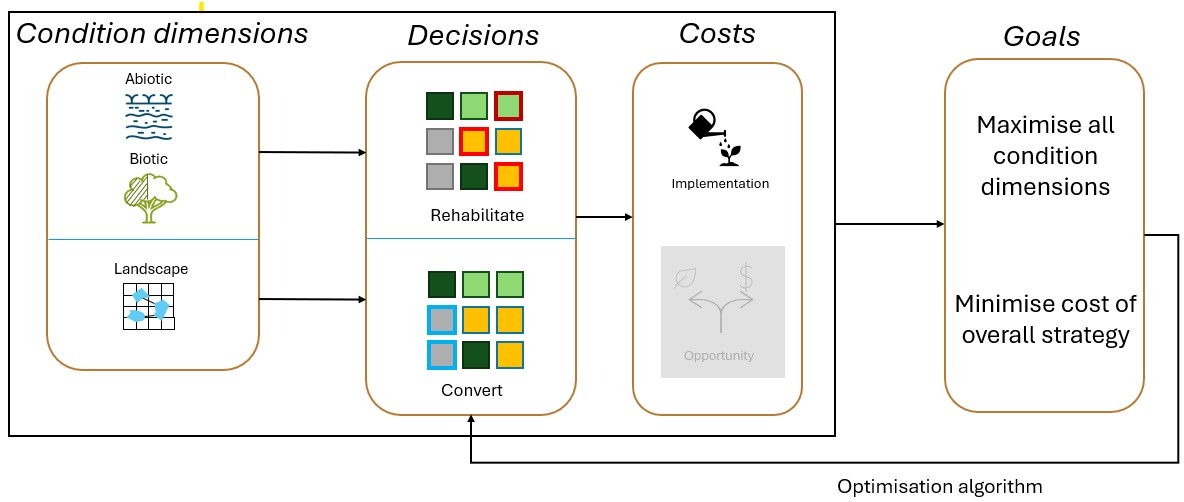
\includegraphics[keepaspectratio]{figs/workflow_feb.jpg}}

\subsection{Initial Conditions}\label{initial-conditions}

\subsubsection{Spatial distribution}\label{spatial-distribution}

\pandocbounded{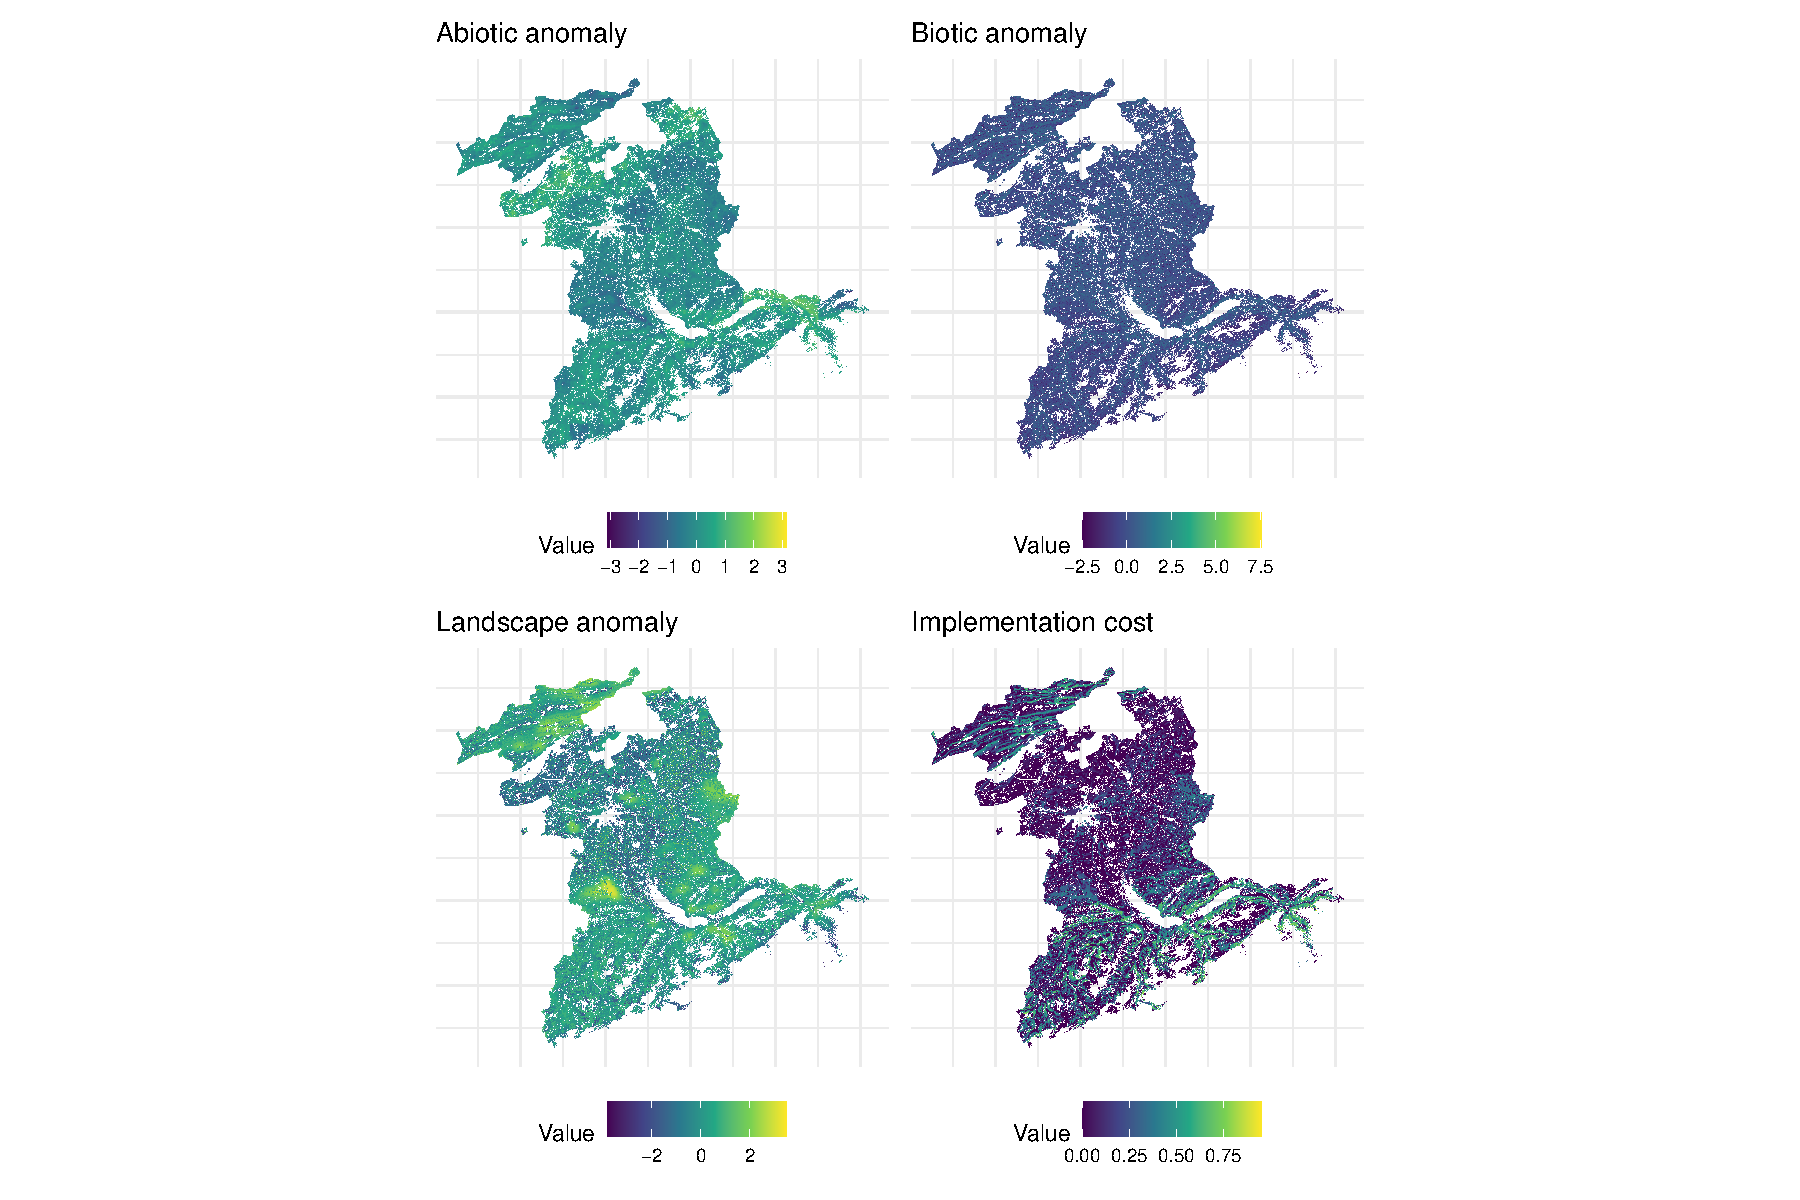
\includegraphics[keepaspectratio]{optimization_results_analysis_files/figure-pdf/initial-conditions-spatial-1.pdf}}

\subsubsection{Distribution of values}\label{distribution-of-values}

\pandocbounded{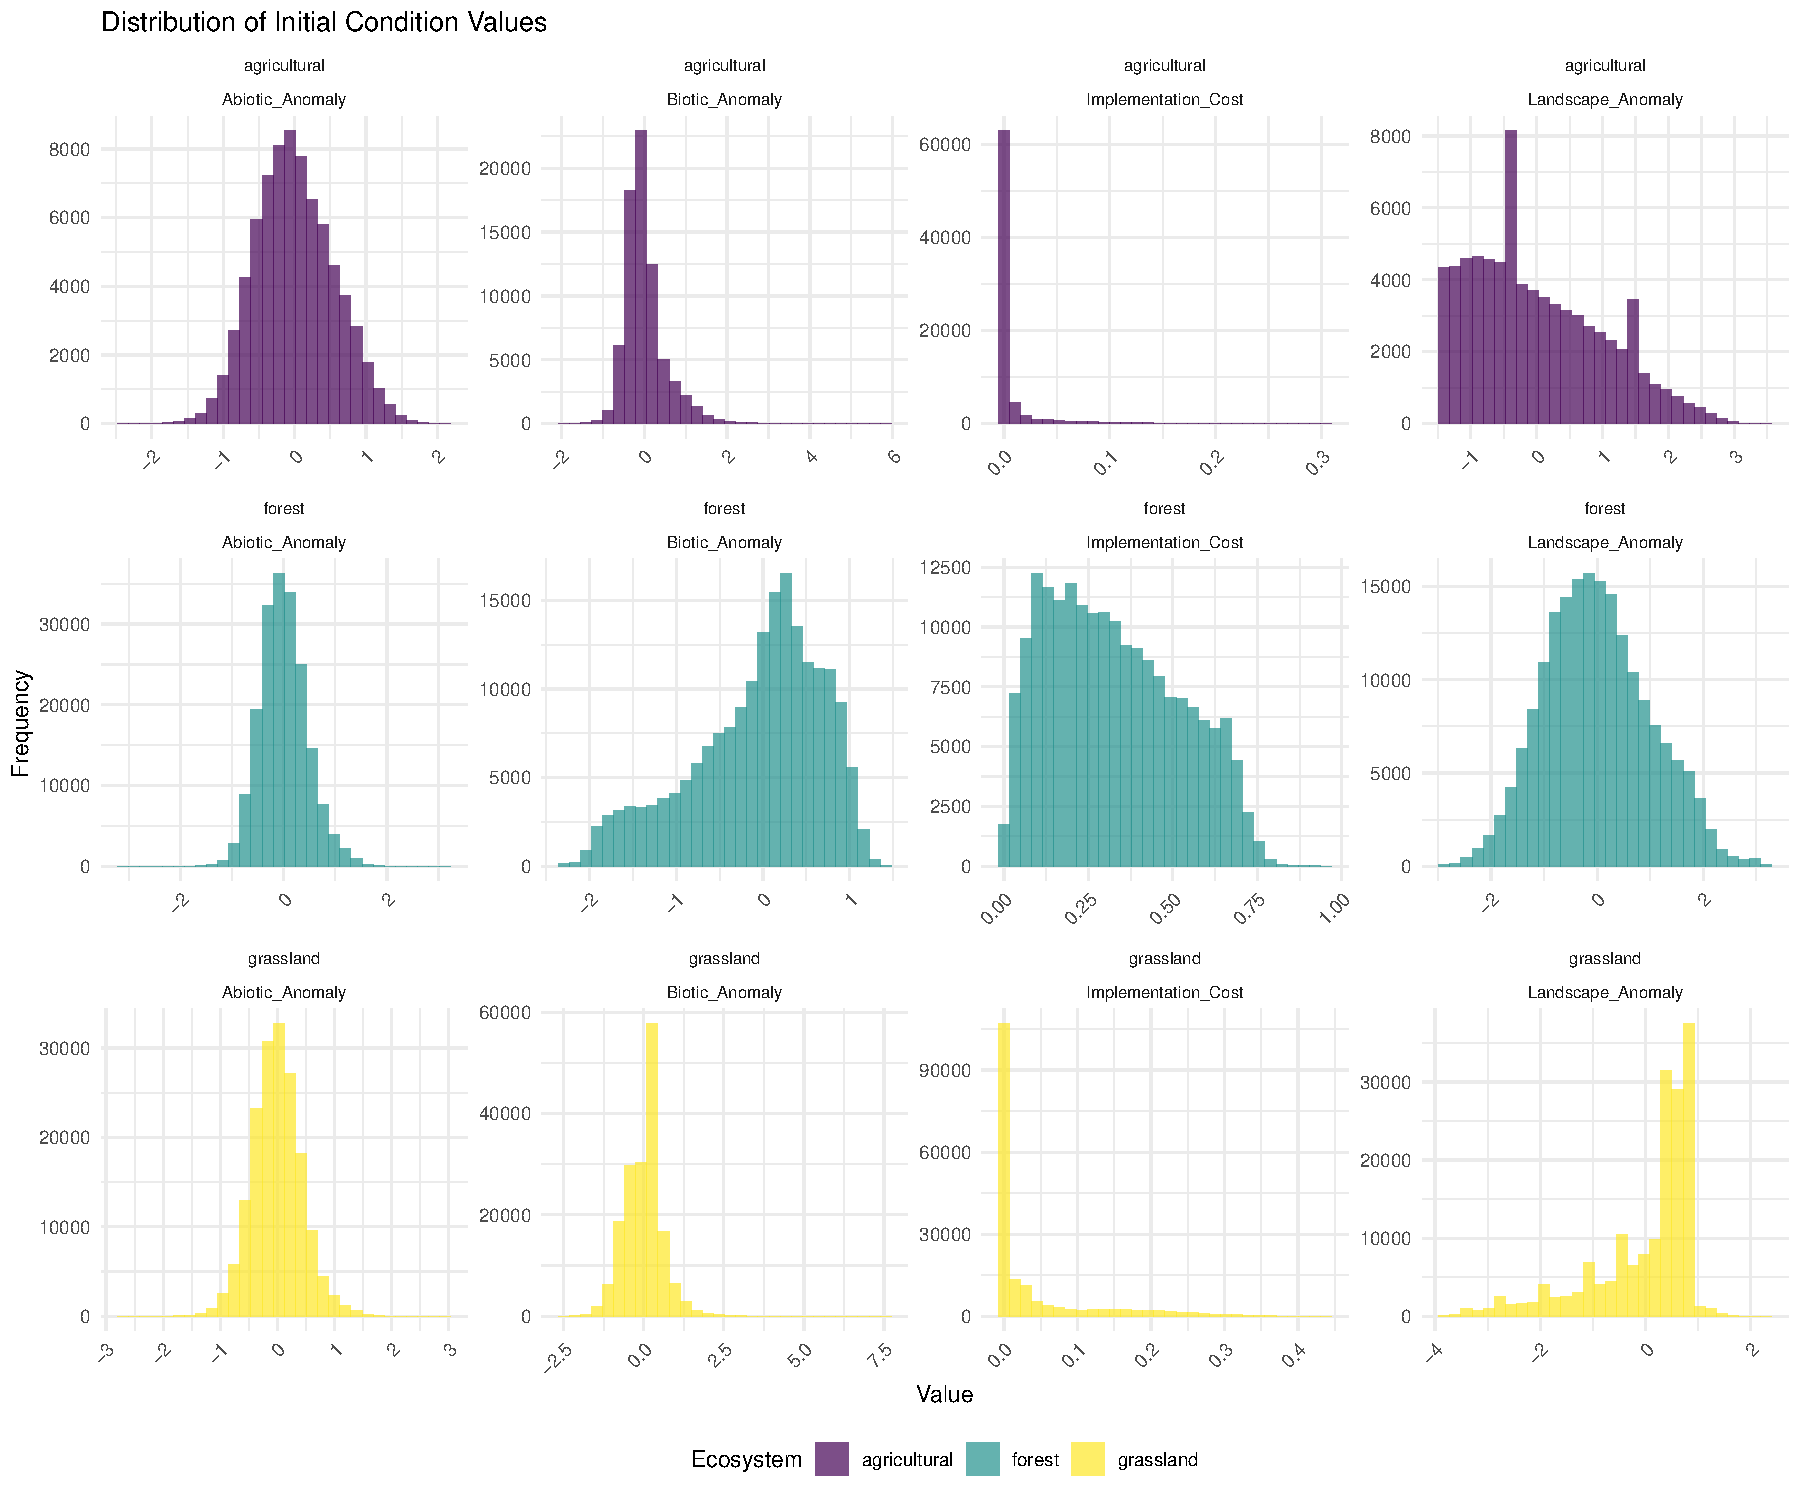
\includegraphics[keepaspectratio]{optimization_results_analysis_files/figure-pdf/initial-conditions-histograms-1.pdf}}

\section{Objectives \& decisions}\label{objectives-decisions}

Decision to restore:

\[
x_i^{R} \in \{0,1\}
\]

Decision to convert:

\[
x_j^{C} \in \{0,1\}
\]

Within a set budget of actions

\[
\sum_i x_i^{R} + \sum_j x_j^{C} = N_{\text{budget}}
\]

\subsection{Overview of objective
functions}\label{overview-of-objective-functions}

\textbf{Abiotic \& biotic condition}

Positive or neutral anomalies receive no improvement. For restored
pixels starting with a negative anomaly: \[
a_i^{1} = a_i^{0} + \alpha_A \, w(a_i^{0})
\]

\begin{itemize}
\tightlist
\item
  \(a_i^{1}\) is the anomaly after restoration, \(a_i^{0}\) is the
  baseline anomaly
\item
  \(\alpha_A\) = abiotic effect, i.e.~a constant that represents an
  arbitrary improvement achieved through restoration
\item
  \(w(a)\) is a weighting function based on the magnitude of the
  anomaly.
\end{itemize}

The improvement is scaled by a weight that depends on the baseline
anomaly. This assigns larger improvement weights to pixels with larger
negative anomalies. If the anomaly is close to zero, the weight is
small. As the anomaly becomes more negative, the weight increases and
approaches 1.

\[
w(a) = \left(1 - e^{-\frac{|a|}{s}}\right)^{\gamma}
\]

\begin{itemize}
\tightlist
\item
  s and \(gamma\) are shape parameters that control how quickly the
  weight increases with the magnitude of the anomaly. Probably both
  aren't needed.
\end{itemize}

\pandocbounded{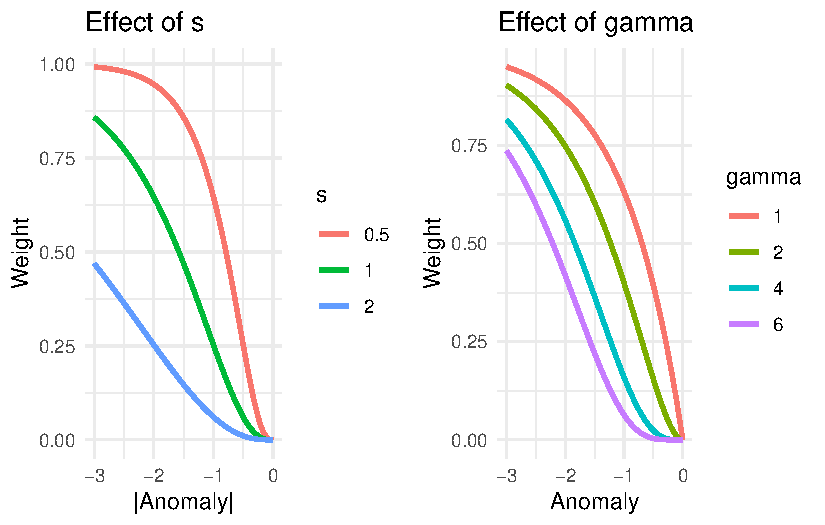
\includegraphics[keepaspectratio]{optimization_results_analysis_files/figure-pdf/unnamed-chunk-1-1.pdf}}

For pixels neighbouring restored pixels: \[
a_k^{1} = a_k^{0} + \alpha_A \, \lambda \, w(a_k^{0})
\]

\begin{itemize}
\tightlist
\item
  \(\lambda\) is the effect decay with distance from the restored pixel.
\end{itemize}

Optimisation minimises the negative total improvement over the study
area (i.e., Maximises total abiotic/biotic improvement from
restoration):

\[
f_{\text{a/biotic}}(x)=-\sum_{i \in \Omega_R}\left(a_i^{1} - a_i^{0}\right)
\]

Other choices for the objective function could be to maximise the
improvement in the worst-off pixels (i.e., minimising the worst anomaly
after restoration), or maximising the number of pixels for which
condition passes a certain threshold.

\textbf{Landscape condition}

\(x_j^{C}\) = 1 changes LULC of selected pixels to a desired class.
Landscape anomaly is recalculated based on new LULC raster.

\[
L^{1} = 1 - D(\mathrm{LULC}^{1})
\]

where \[
\mathrm{LULC}^{1} =\begin{cases}\text{focal class}, & \text{if } x_j^{C} = 1 \\\mathrm{LULC}^{0}, & \text{otherwise}\end{cases}
\]

Optimisation minimises the total landscape anomaly across the whole
study area:

\[
f_{\text{landscape}}(x) =\sum_{p \in \Omega}L_p^{1}
\]

Optimisation minimizes the total landscape anomaly as the simple sum of
the landscape anomaly raster values after applying the conversion driven
landscape update.

\textbf{Implementation cost}

\[
f_{\text{cost}}(x) =\sum_{k \in \Omega_{R}} y^{R}_{k}(x)\,c_{k}+\sum_{k \in \Omega_{C}} y^{C}_{k}(x)\,c_{k}
\]

The code computes total implementation cost as the sum of baseline cost
over all pixels selected for restoration plus all pixels selected for
conversion, then minimizes that total.

\textbf{Baseline values}

\pandocbounded{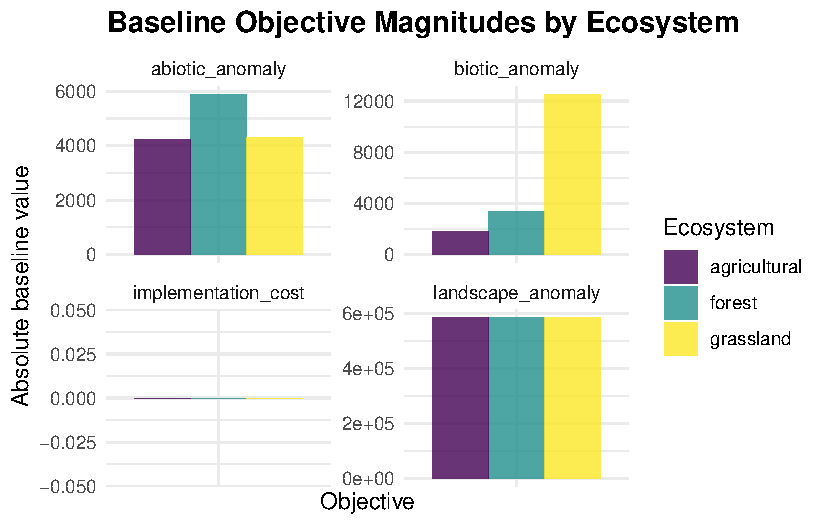
\includegraphics[keepaspectratio]{optimization_results_analysis_files/figure-pdf/baseline-data-viz-1.pdf}}

Calculation of the landscape anomaly same for each ecosystem type,
because the calculation is the same\ldots logically this might need some
work. Implementation cost objective is 0 for all ecosystems, as cost
only incurred after restoration decisions are applied.

\subsection{Eligible pixels for restoration and
conversion}\label{eligible-pixels-for-restoration-and-conversion}

\pandocbounded{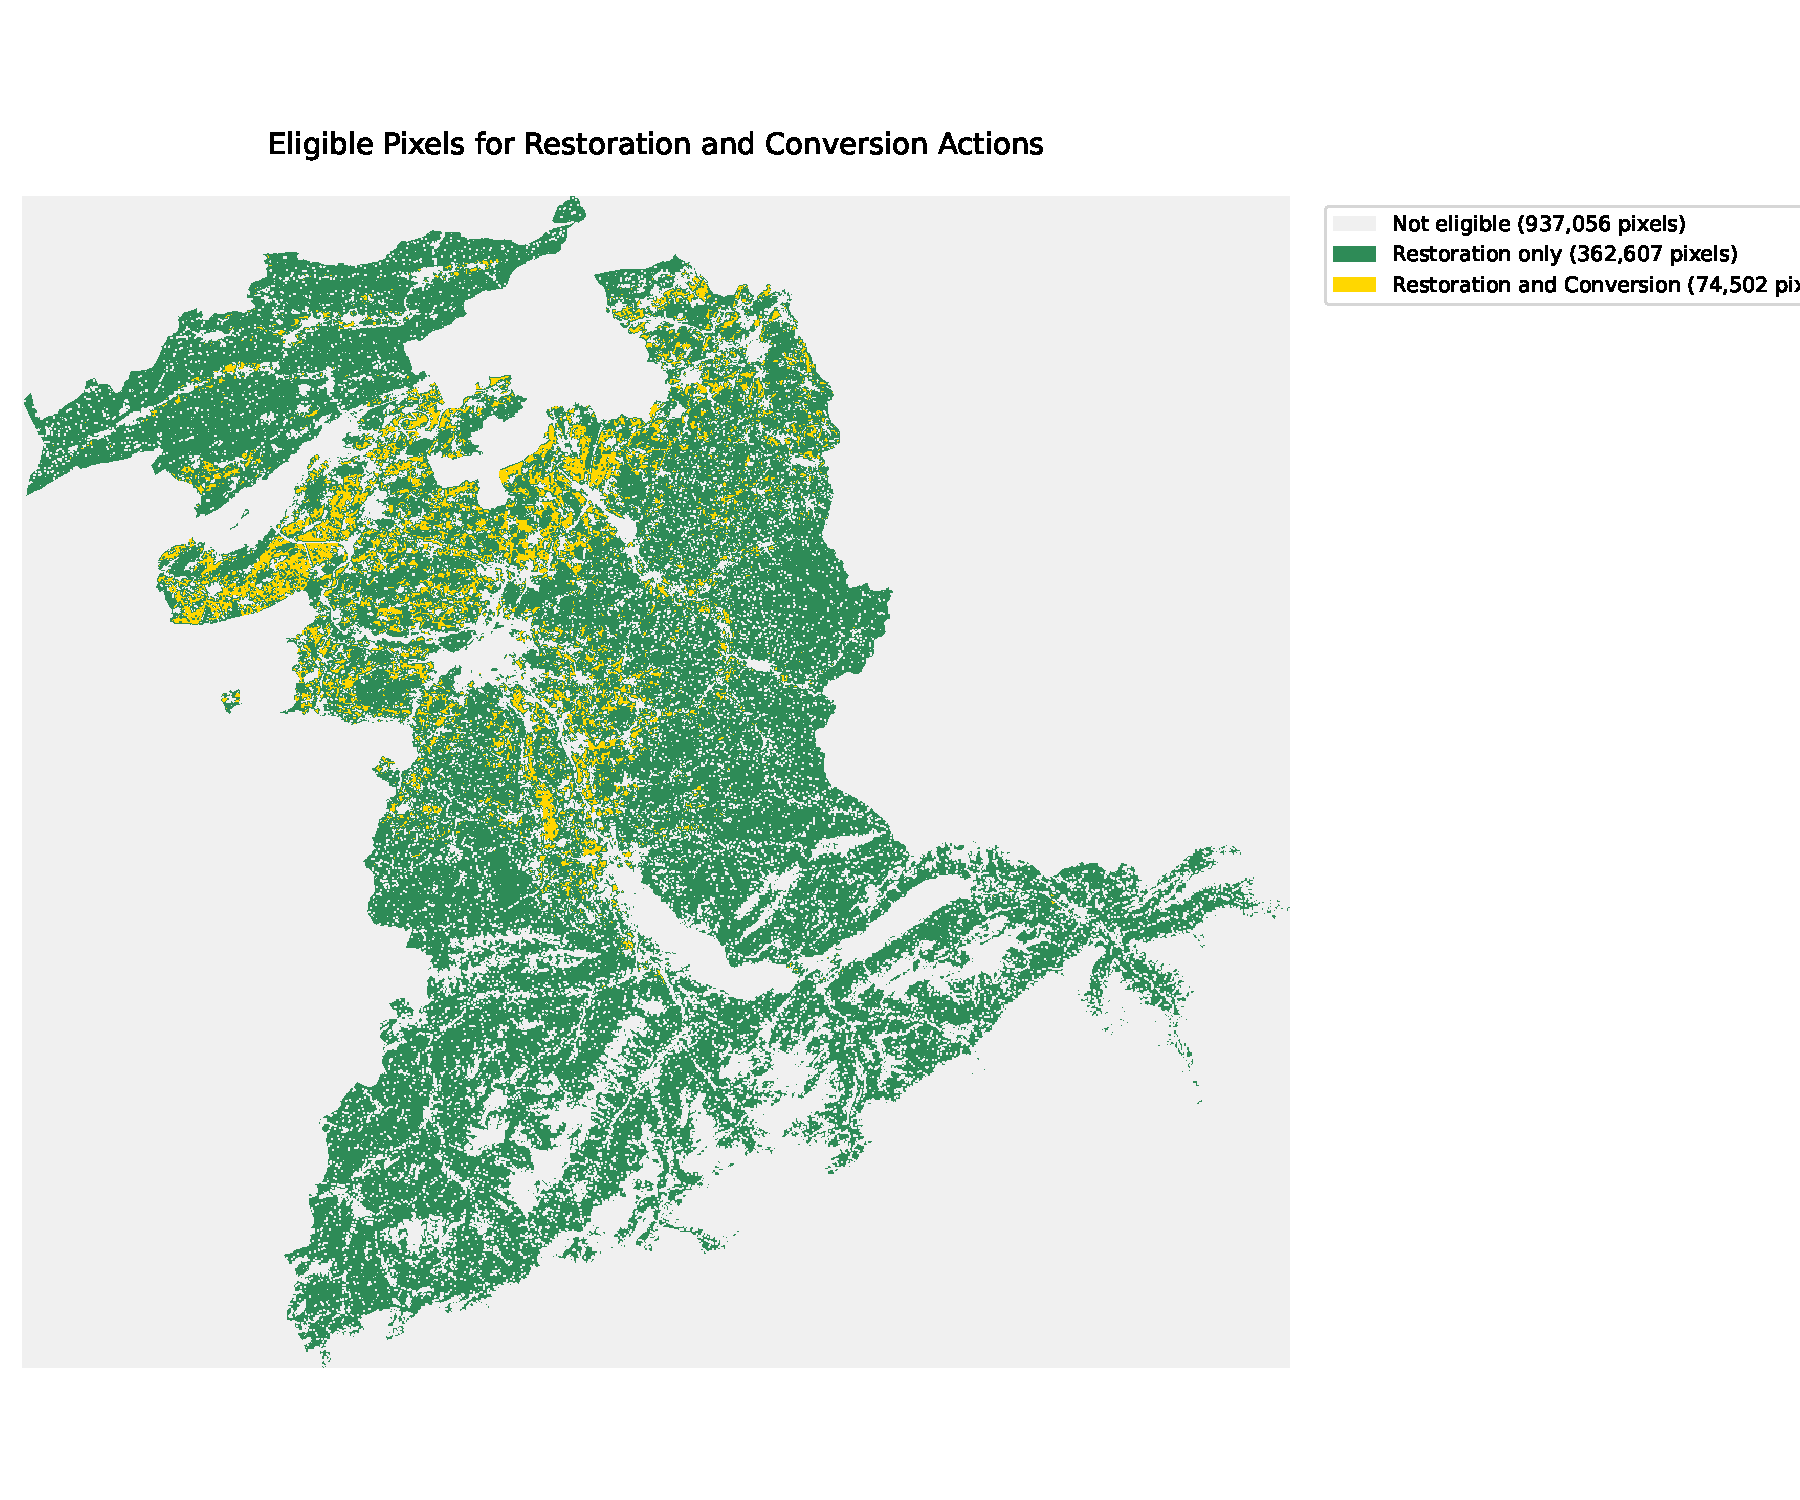
\includegraphics[keepaspectratio]{optimization_results_analysis_files/figure-pdf/eligible-pixels-viz-1.pdf}}

Pixels eligible for restoration: any pixels within the ecosystem type
(Forest: Open \& Closed Forest; Agricultural: Intensive Agriculture;
Grassland: Grassland \& Alpine Pastures)

\subsection{Constraints and repair}\label{constraints-and-repair}

\emph{Constraint formulation}

The optimisation is formulated with a fixed restoration budget.

The total number of selected pixels, including restoration and
conversion actions, is constrained to equal a predefined maximum derived
from the scenario specific restoration fraction.

\emph{Repair strategy}

A unified adaptive repair operator is applied after crossover and
mutation.

\begin{itemize}
\tightlist
\item
  Solutions that deviate strongly from the target number of actions
  (\textgreater20\% of target number) are adjusted to restore
  feasibility.
\item
  Small deviations are tolerated to preserve diversity.
\item
  When repair is required, pixels are added or removed using a neutral,
  random mechanism.
\end{itemize}

\section{Output from optimisation
runs}\label{output-from-optimisation-runs}

\subsection{Overview by Ecosystem}\label{overview-by-ecosystem}

\begin{longtable}[]{@{}lrrr@{}}
\caption{Summary by ecosystem}\tabularnewline
\toprule\noalign{}
Metric & forest & agricultural & grassland \\
\midrule\noalign{}
\endfirsthead
\toprule\noalign{}
Metric & forest & agricultural & grassland \\
\midrule\noalign{}
\endhead
\bottomrule\noalign{}
\endlastfoot
Objectives & 4.00 & 4.00 & 4.00 \\
Total\_Pixels & 49567.00 & 28921.00 & 42481.00 \\
Max\_Restored\_Pixels & 4956.00 & 2892.00 & 4248.00 \\
Max\_Restoration\_fraction & 0.10 & 0.10 & 0.10 \\
Population\_Size & 20.00 & 20.00 & 20.00 \\
Actual\_Generations & 30.00 & 30.00 & 30.00 \\
Pareto\_Solutions & 20.00 & 20.00 & 18.00 \\
Final\_Hypervolume & 14812.07 & 48.84 & 166.12 \\
\end{longtable}

\subsubsection{Objective Statistics Comparison Across
Ecosystems}\label{objective-statistics-comparison-across-ecosystems}

\begin{longtable}[]{@{}
  >{\raggedright\arraybackslash}p{(\linewidth - 14\tabcolsep) * \real{0.1529}}
  >{\raggedright\arraybackslash}p{(\linewidth - 14\tabcolsep) * \real{0.2353}}
  >{\raggedleft\arraybackslash}p{(\linewidth - 14\tabcolsep) * \real{0.0941}}
  >{\raggedleft\arraybackslash}p{(\linewidth - 14\tabcolsep) * \real{0.1176}}
  >{\raggedleft\arraybackslash}p{(\linewidth - 14\tabcolsep) * \real{0.1059}}
  >{\raggedleft\arraybackslash}p{(\linewidth - 14\tabcolsep) * \real{0.1059}}
  >{\raggedleft\arraybackslash}p{(\linewidth - 14\tabcolsep) * \real{0.1059}}
  >{\raggedleft\arraybackslash}p{(\linewidth - 14\tabcolsep) * \real{0.0824}}@{}}
\caption{Objective Statistics Comparison Across
Ecosystems}\tabularnewline
\toprule\noalign{}
\begin{minipage}[b]{\linewidth}\raggedright
Ecosystem
\end{minipage} & \begin{minipage}[b]{\linewidth}\raggedright
Objective
\end{minipage} & \begin{minipage}[b]{\linewidth}\raggedleft
Min
\end{minipage} & \begin{minipage}[b]{\linewidth}\raggedleft
Max
\end{minipage} & \begin{minipage}[b]{\linewidth}\raggedleft
Mean
\end{minipage} & \begin{minipage}[b]{\linewidth}\raggedleft
Std
\end{minipage} & \begin{minipage}[b]{\linewidth}\raggedleft
Range
\end{minipage} & \begin{minipage}[b]{\linewidth}\raggedleft
CV
\end{minipage} \\
\midrule\noalign{}
\endfirsthead
\toprule\noalign{}
\begin{minipage}[b]{\linewidth}\raggedright
Ecosystem
\end{minipage} & \begin{minipage}[b]{\linewidth}\raggedright
Objective
\end{minipage} & \begin{minipage}[b]{\linewidth}\raggedleft
Min
\end{minipage} & \begin{minipage}[b]{\linewidth}\raggedleft
Max
\end{minipage} & \begin{minipage}[b]{\linewidth}\raggedleft
Mean
\end{minipage} & \begin{minipage}[b]{\linewidth}\raggedleft
Std
\end{minipage} & \begin{minipage}[b]{\linewidth}\raggedleft
Range
\end{minipage} & \begin{minipage}[b]{\linewidth}\raggedleft
CV
\end{minipage} \\
\midrule\noalign{}
\endhead
\bottomrule\noalign{}
\endlastfoot
forest & abiotic\_anomaly & -2.8207 & -0.0607 & -1.6428 & 0.7848 &
2.7600 & 0.4777 \\
forest & biotic\_anomaly & -8.5937 & -0.1859 & -4.6057 & 2.4186 & 8.4079
& 0.5251 \\
forest & landscape\_anomaly & 1.2917 & 1.3001 & 1.2957 & 0.0025 & 0.0083
& 0.0019 \\
forest & implementation\_cost & 48.0717 & 1008.5867 & 508.7992 &
286.7973 & 960.5149 & 0.5637 \\
agricultural & abiotic\_anomaly & -2.6546 & -0.0484 & -1.6659 & 0.7722 &
2.6062 & 0.4636 \\
agricultural & biotic\_anomaly & -0.8992 & -0.0280 & -0.5696 & 0.2547 &
0.8712 & 0.4471 \\
agricultural & landscape\_anomaly & 1.2953 & 1.2999 & 1.2978 & 0.0014 &
0.0047 & 0.0011 \\
agricultural & implementation\_cost & 18.2450 & 24.7198 & 21.1812 &
1.7457 & 6.4749 & 0.0824 \\
grassland & abiotic\_anomaly & -1.8818 & -0.5242 & -1.2246 & 0.4272 &
1.3576 & 0.3489 \\
grassland & biotic\_anomaly & -0.2748 & -0.0846 & -0.1875 & 0.0612 &
0.1902 & 0.3263 \\
grassland & landscape\_anomaly & 1.2943 & 1.3000 & 1.2971 & 0.0018 &
0.0056 & 0.0014 \\
grassland & implementation\_cost & 48.3649 & 136.1754 & 92.1121 &
26.6714 & 87.8104 & 0.2896 \\
\end{longtable}

\subsubsection{Decisions}\label{decisions}

(choice to restore vs convert)

\begin{longtable}[]{@{}
  >{\raggedright\arraybackslash}p{(\linewidth - 30\tabcolsep) * \real{0.0610}}
  >{\raggedleft\arraybackslash}p{(\linewidth - 30\tabcolsep) * \real{0.0563}}
  >{\raggedleft\arraybackslash}p{(\linewidth - 30\tabcolsep) * \real{0.0563}}
  >{\raggedleft\arraybackslash}p{(\linewidth - 30\tabcolsep) * \real{0.0610}}
  >{\raggedleft\arraybackslash}p{(\linewidth - 30\tabcolsep) * \real{0.0563}}
  >{\raggedleft\arraybackslash}p{(\linewidth - 30\tabcolsep) * \real{0.0563}}
  >{\raggedleft\arraybackslash}p{(\linewidth - 30\tabcolsep) * \real{0.0563}}
  >{\raggedleft\arraybackslash}p{(\linewidth - 30\tabcolsep) * \real{0.0610}}
  >{\raggedleft\arraybackslash}p{(\linewidth - 30\tabcolsep) * \real{0.0563}}
  >{\raggedleft\arraybackslash}p{(\linewidth - 30\tabcolsep) * \real{0.0469}}
  >{\raggedleft\arraybackslash}p{(\linewidth - 30\tabcolsep) * \real{0.0469}}
  >{\raggedleft\arraybackslash}p{(\linewidth - 30\tabcolsep) * \real{0.0516}}
  >{\raggedleft\arraybackslash}p{(\linewidth - 30\tabcolsep) * \real{0.0469}}
  >{\raggedleft\arraybackslash}p{(\linewidth - 30\tabcolsep) * \real{0.1080}}
  >{\raggedleft\arraybackslash}p{(\linewidth - 30\tabcolsep) * \real{0.1033}}
  >{\raggedleft\arraybackslash}p{(\linewidth - 30\tabcolsep) * \real{0.0751}}@{}}
\caption{Decision Pattern Statistics by Ecosystem}\tabularnewline
\toprule\noalign{}
\begin{minipage}[b]{\linewidth}\raggedright
Ecosystem
\end{minipage} & \begin{minipage}[b]{\linewidth}\raggedleft
Restore\_Min
\end{minipage} & \begin{minipage}[b]{\linewidth}\raggedleft
Restore\_Max
\end{minipage} & \begin{minipage}[b]{\linewidth}\raggedleft
Restore\_Mean
\end{minipage} & \begin{minipage}[b]{\linewidth}\raggedleft
Restore\_Std
\end{minipage} & \begin{minipage}[b]{\linewidth}\raggedleft
Convert\_Min
\end{minipage} & \begin{minipage}[b]{\linewidth}\raggedleft
Convert\_Max
\end{minipage} & \begin{minipage}[b]{\linewidth}\raggedleft
Convert\_Mean
\end{minipage} & \begin{minipage}[b]{\linewidth}\raggedleft
Convert\_Std
\end{minipage} & \begin{minipage}[b]{\linewidth}\raggedleft
Total\_Min
\end{minipage} & \begin{minipage}[b]{\linewidth}\raggedleft
Total\_Max
\end{minipage} & \begin{minipage}[b]{\linewidth}\raggedleft
Total\_Mean
\end{minipage} & \begin{minipage}[b]{\linewidth}\raggedleft
Total\_Std
\end{minipage} & \begin{minipage}[b]{\linewidth}\raggedleft
Max\_Restoration\_Pixels
\end{minipage} & \begin{minipage}[b]{\linewidth}\raggedleft
Max\_Conversion\_Pixels
\end{minipage} & \begin{minipage}[b]{\linewidth}\raggedleft
Budget\_Fraction
\end{minipage} \\
\midrule\noalign{}
\endfirsthead
\toprule\noalign{}
\begin{minipage}[b]{\linewidth}\raggedright
Ecosystem
\end{minipage} & \begin{minipage}[b]{\linewidth}\raggedleft
Restore\_Min
\end{minipage} & \begin{minipage}[b]{\linewidth}\raggedleft
Restore\_Max
\end{minipage} & \begin{minipage}[b]{\linewidth}\raggedleft
Restore\_Mean
\end{minipage} & \begin{minipage}[b]{\linewidth}\raggedleft
Restore\_Std
\end{minipage} & \begin{minipage}[b]{\linewidth}\raggedleft
Convert\_Min
\end{minipage} & \begin{minipage}[b]{\linewidth}\raggedleft
Convert\_Max
\end{minipage} & \begin{minipage}[b]{\linewidth}\raggedleft
Convert\_Mean
\end{minipage} & \begin{minipage}[b]{\linewidth}\raggedleft
Convert\_Std
\end{minipage} & \begin{minipage}[b]{\linewidth}\raggedleft
Total\_Min
\end{minipage} & \begin{minipage}[b]{\linewidth}\raggedleft
Total\_Max
\end{minipage} & \begin{minipage}[b]{\linewidth}\raggedleft
Total\_Mean
\end{minipage} & \begin{minipage}[b]{\linewidth}\raggedleft
Total\_Std
\end{minipage} & \begin{minipage}[b]{\linewidth}\raggedleft
Max\_Restoration\_Pixels
\end{minipage} & \begin{minipage}[b]{\linewidth}\raggedleft
Max\_Conversion\_Pixels
\end{minipage} & \begin{minipage}[b]{\linewidth}\raggedleft
Budget\_Fraction
\end{minipage} \\
\midrule\noalign{}
\endhead
\bottomrule\noalign{}
\endlastfoot
forest & 61 & 4926 & 2371.40 & 1437.13 & 30 & 4895 & 2584.60 & 1437.13 &
4956 & 4956 & 4956 & 0 & 49567 & 38025 & 0.1 \\
agricultural & 51 & 2766 & 1547.10 & 823.25 & 126 & 2841 & 1344.90 &
823.25 & 2892 & 2892 & 2892 & 0 & 28921 & 28921 & 0.1 \\
grassland & 860 & 4149 & 2462.44 & 1059.42 & 99 & 3388 & 1785.56 &
1059.42 & 4248 & 4248 & 4248 & 0 & 42481 & 38177 & 0.1 \\
\end{longtable}

\section{Issues/debugging of optimisation
results}\label{issuesdebugging-of-optimisation-results}

\subsection{A: Weak spatial signal in
selection}\label{a-weak-spatial-signal-in-selection}

\subsubsection{Selection Frequency Maps}\label{selection-frequency-maps}

(small error in the pixel counts on these plots)

\pandocbounded{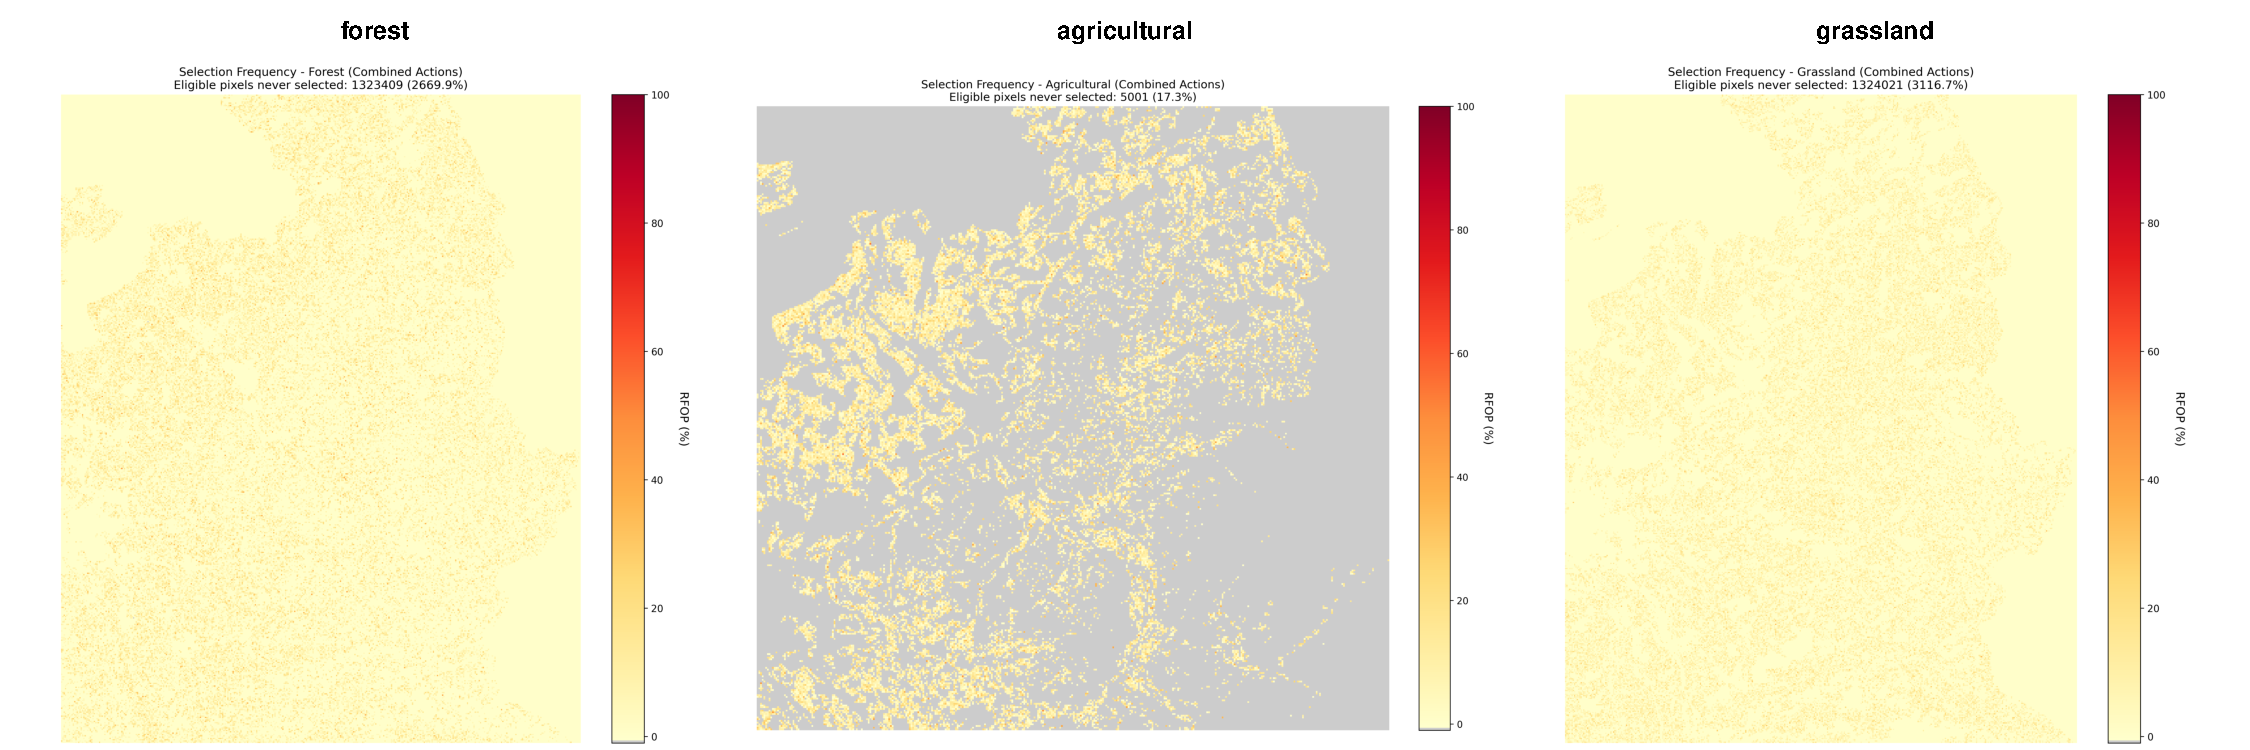
\includegraphics[keepaspectratio]{optimization_results_analysis_files/figure-pdf/selection-frequency-grid-25.pdf}}

\subsubsection{Example Pareto-Optimal
Solutions}\label{example-pareto-optimal-solutions}

\pandocbounded{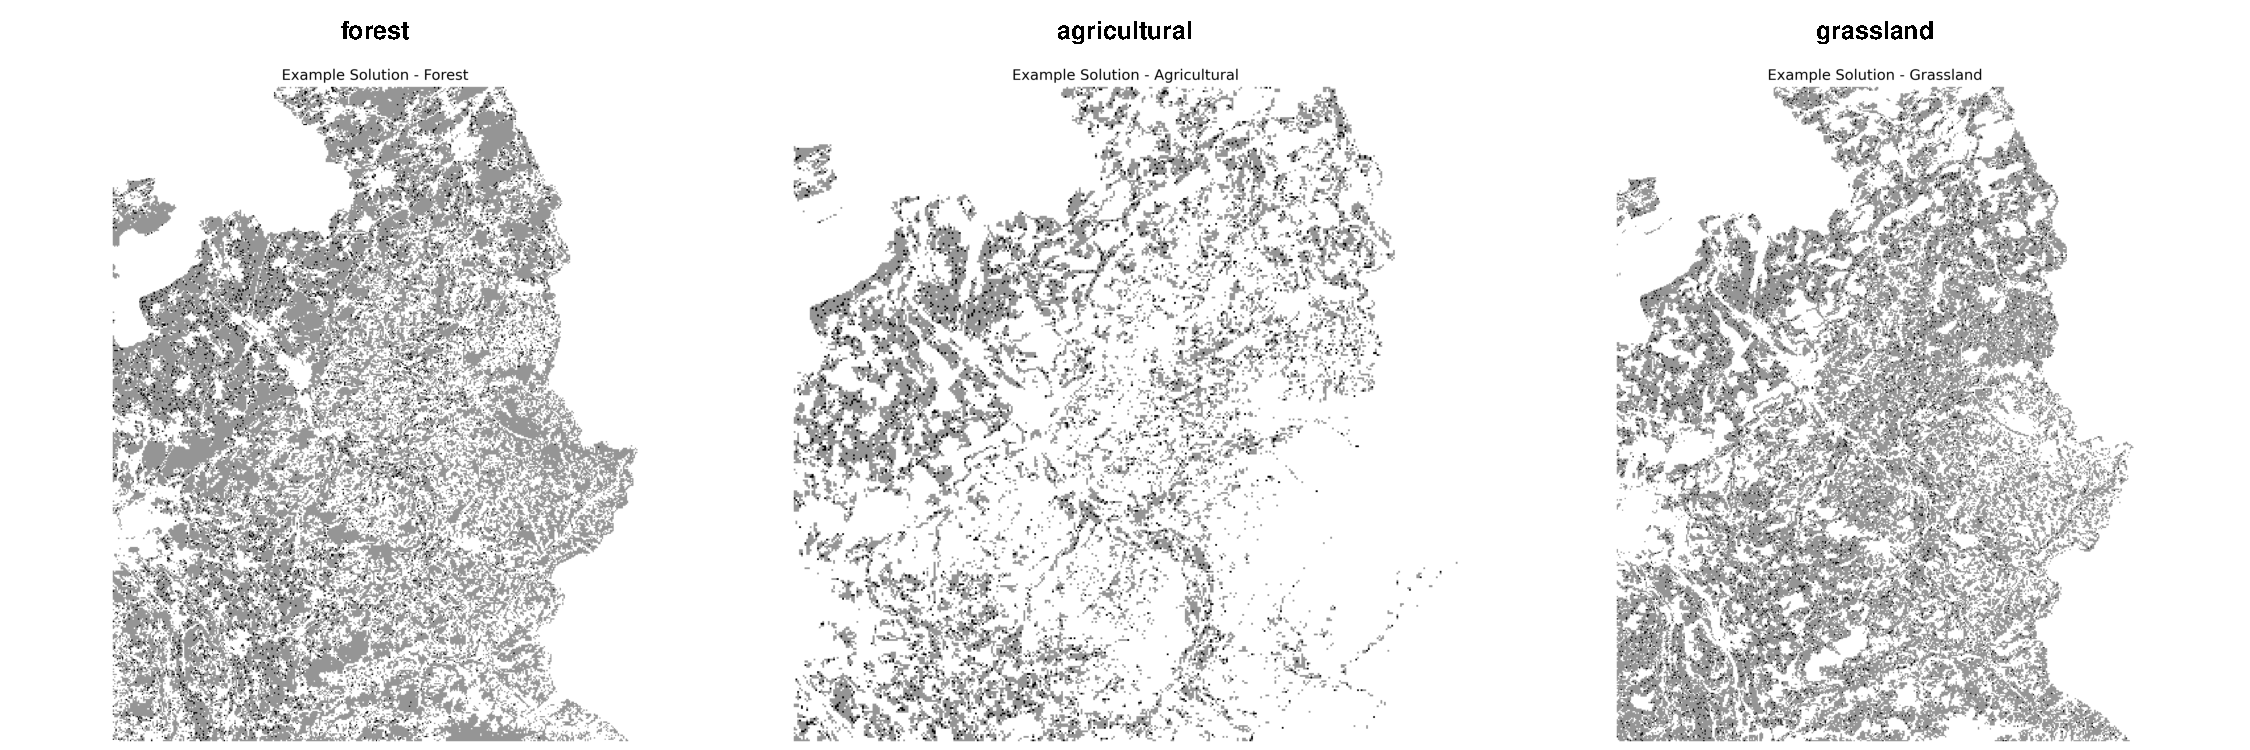
\includegraphics[keepaspectratio]{optimization_results_analysis_files/figure-pdf/example-solution-grid-1.pdf}}

\subsection{B: Objective space
problems}\label{b-objective-space-problems}

\subsection{B1: Redundancy of
objectives}\label{b1-redundancy-of-objectives}

Cause identified - this is only because the landscape objective is not
well implemented

\subsubsection{Pareto fronts}\label{pareto-fronts}

\pandocbounded{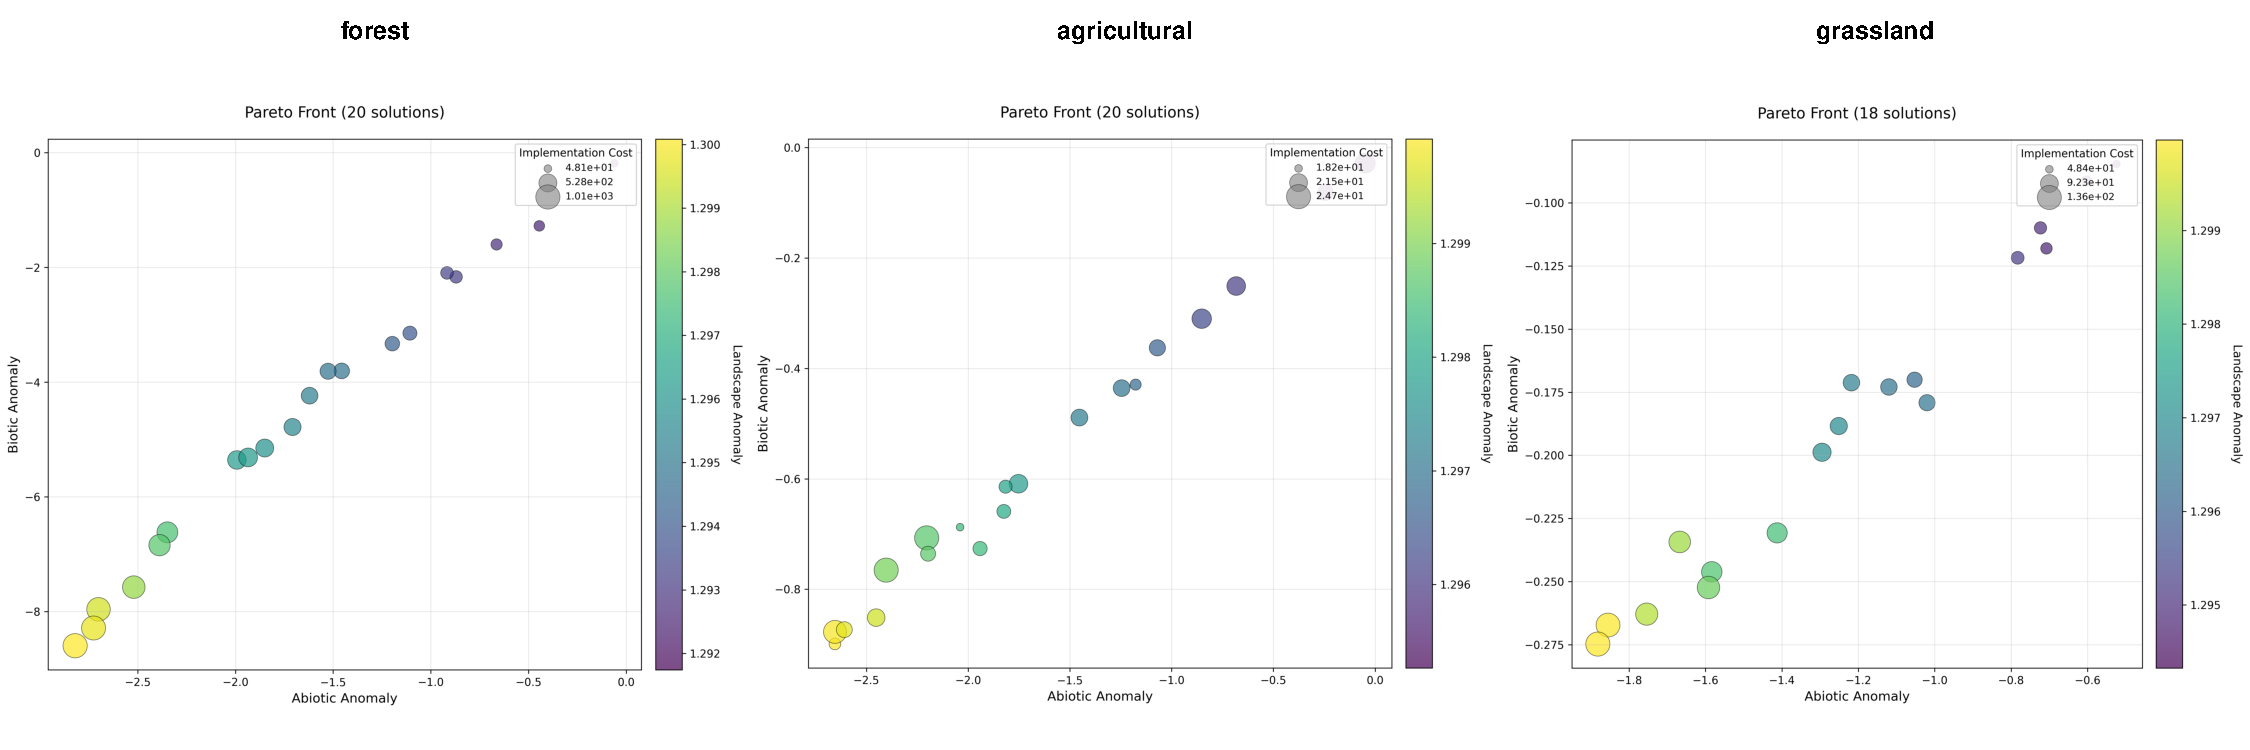
\includegraphics[keepaspectratio]{optimization_results_analysis_files/figure-pdf/pareto-front-grid-1.pdf}}

\subsubsection{Parallel coordinates}\label{parallel-coordinates}

\pandocbounded{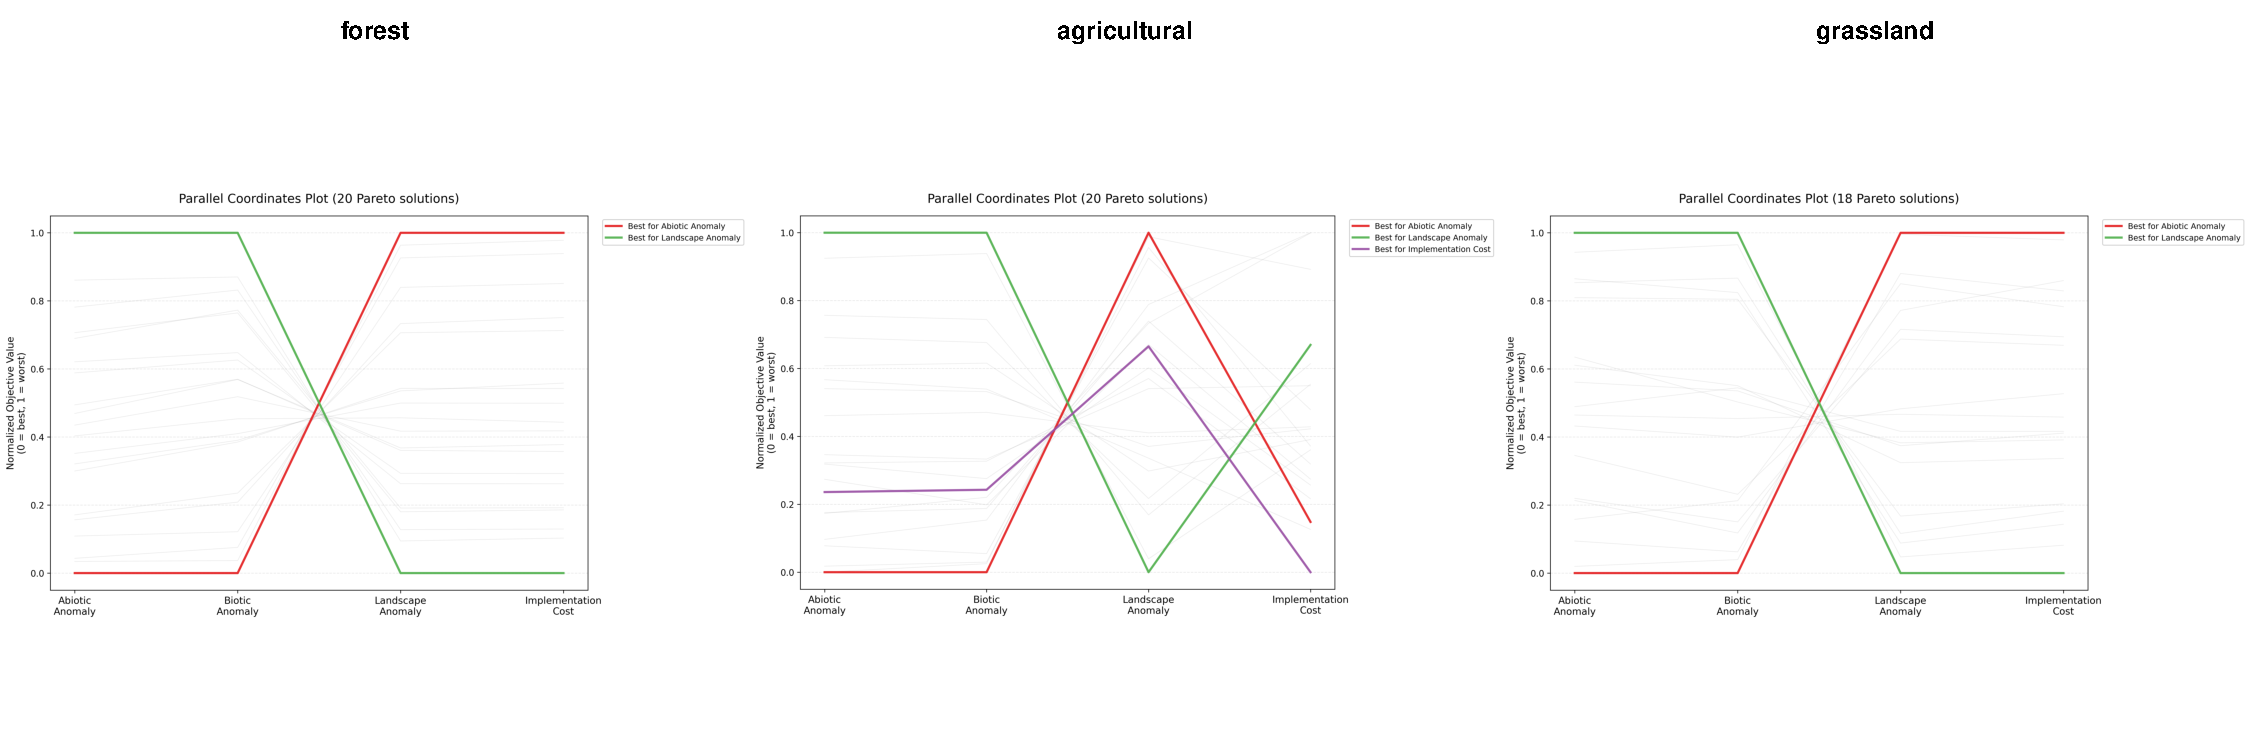
\includegraphics[keepaspectratio]{optimization_results_analysis_files/figure-pdf/parallel-coordinates-grid-1.pdf}}

\subsubsection{Objective correlations}\label{objective-correlations}

\pandocbounded{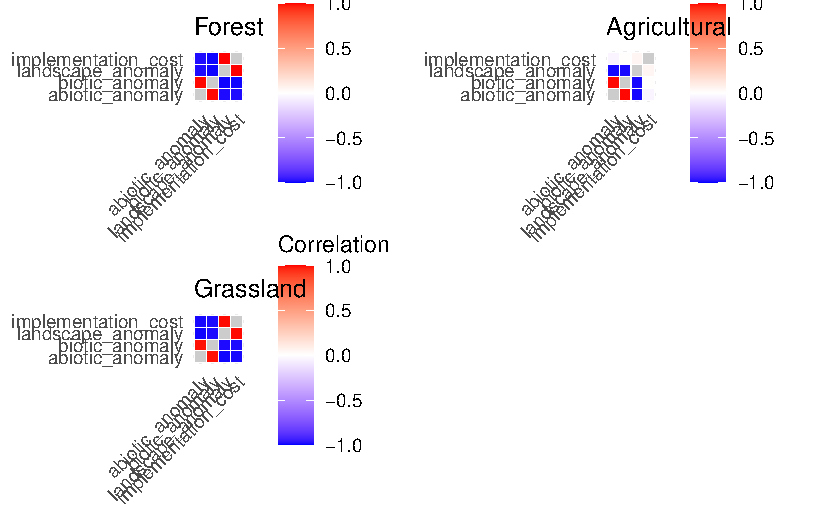
\includegraphics[keepaspectratio]{optimization_results_analysis_files/figure-pdf/correlation-analysis-1.pdf}}

\subsection{Without landscape
objective:}\label{without-landscape-objective}

Running \emph{without} landscape objective --\textgreater{} less
solutions, higher diversity in solutions, weaker correlations between
objectives

\subsubsection{Pareto fronts}\label{pareto-fronts-1}

\pandocbounded{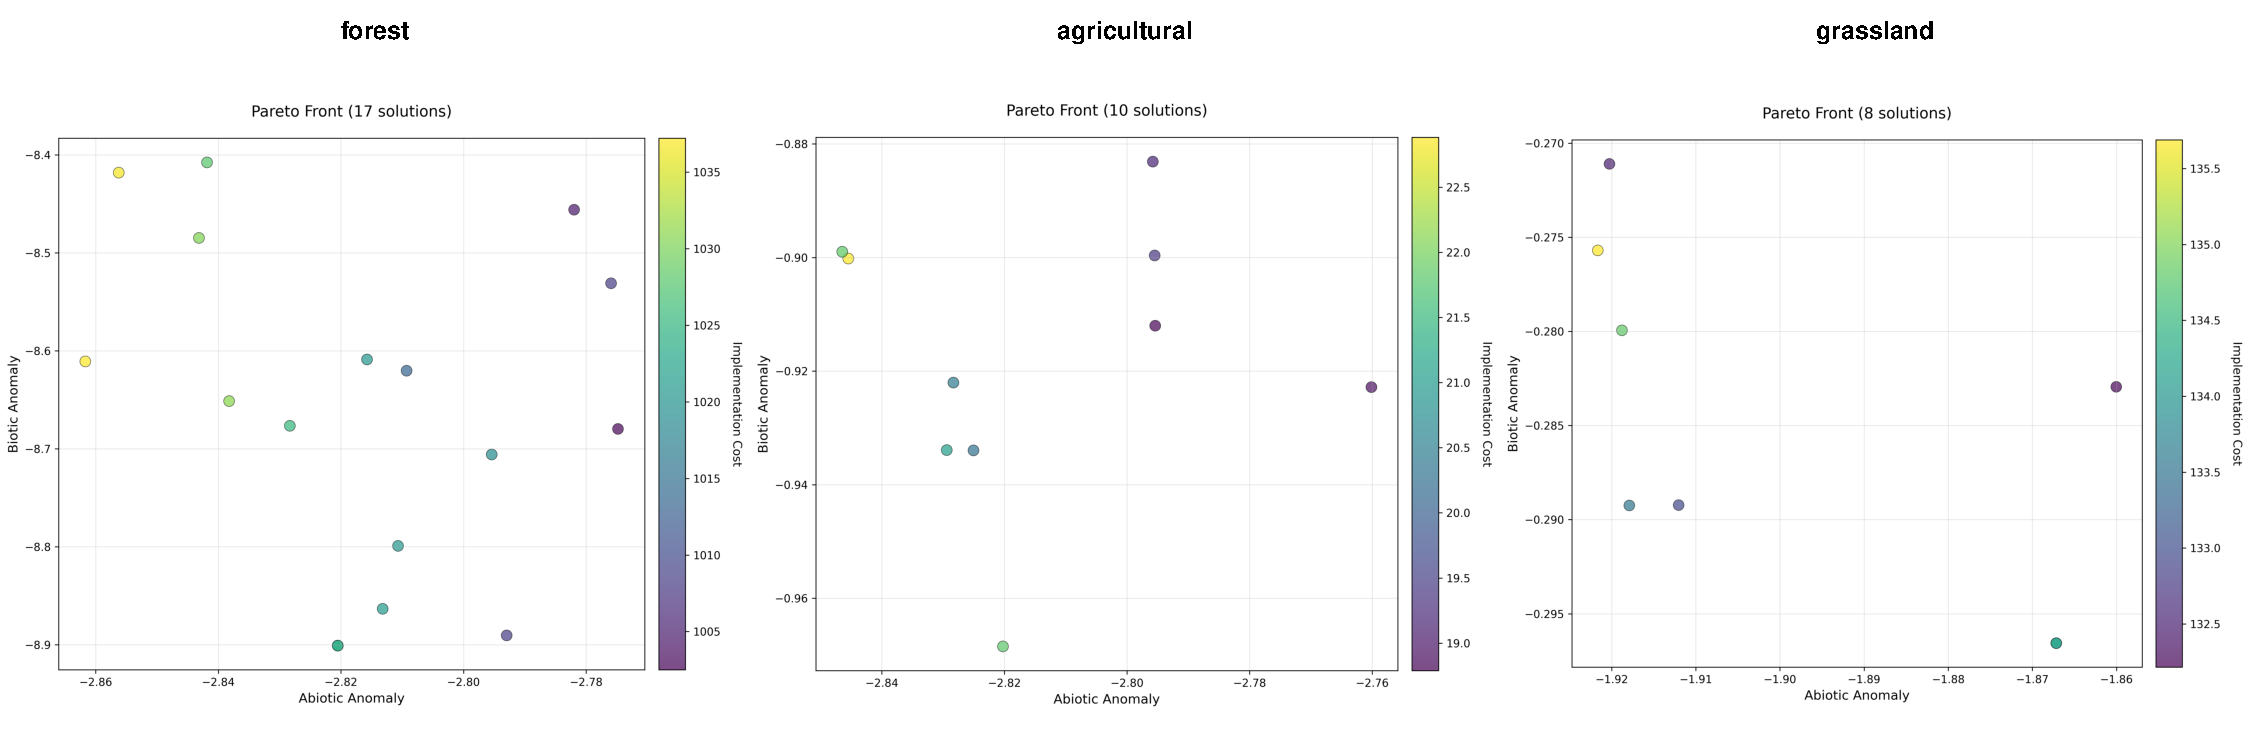
\includegraphics[keepaspectratio]{optimization_results_analysis_files/figure-pdf/pareto-front-grid-ab-1.pdf}}

\subsubsection{Parallel coordinates}\label{parallel-coordinates-1}

\pandocbounded{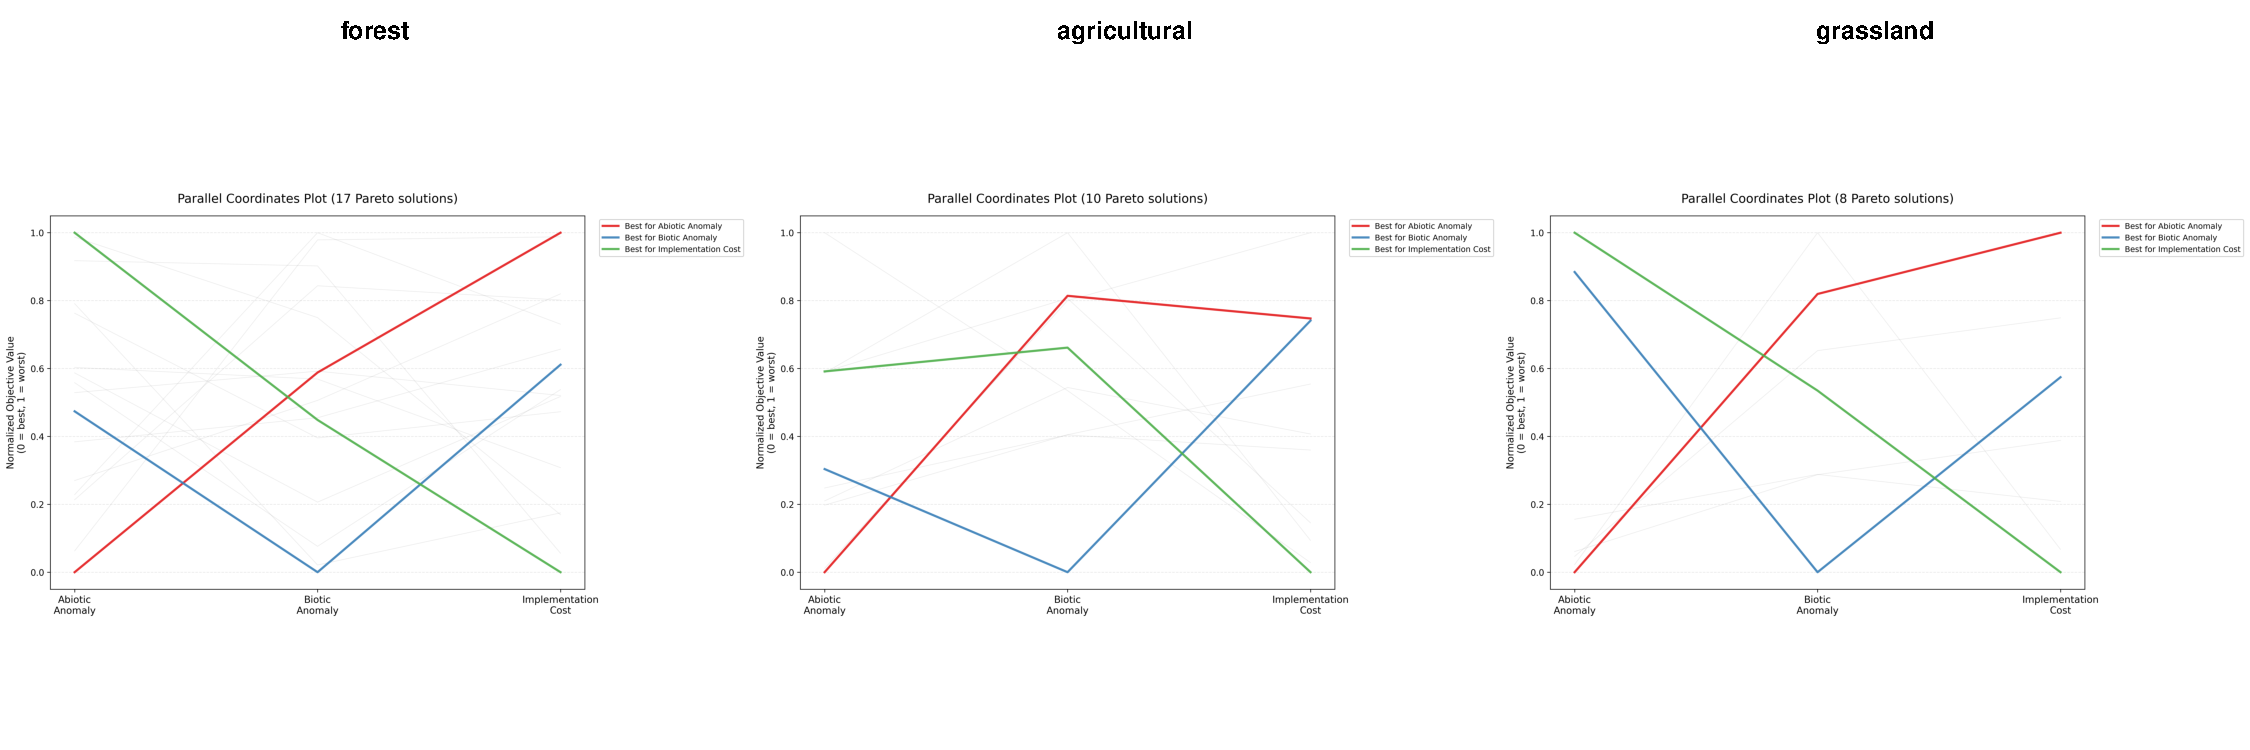
\includegraphics[keepaspectratio]{optimization_results_analysis_files/figure-pdf/parallel-coordinates-grid-ab-1.pdf}}

\subsubsection{Objective correlations}\label{objective-correlations-1}

\pandocbounded{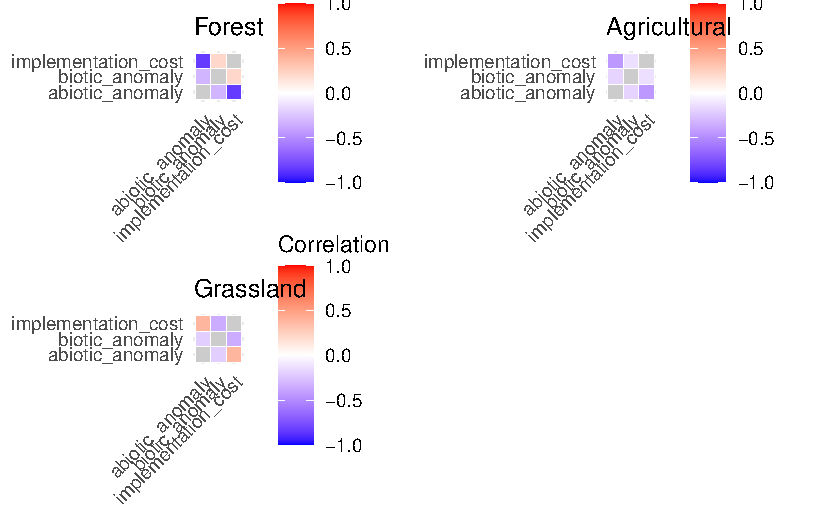
\includegraphics[keepaspectratio]{optimization_results_analysis_files/figure-pdf/correlation-analysis-ab-1.pdf}}

\subsection{B2: Weak sensitivity of landscape
objective}\label{b2-weak-sensitivity-of-landscape-objective}

Basically the current set up of this objective drives very little change
in landscape anomaly values across the solution space, so it has very
little influence on selection of solutions. CV of landscape objective in
all ecosystems is very low.

\subsubsection{Landscape Objective Sensitivity
Test}\label{landscape-objective-sensitivity-test}

\begin{verbatim}
Sampled 100x100 area with 1259 eligible pixels for conversion
\end{verbatim}

\pandocbounded{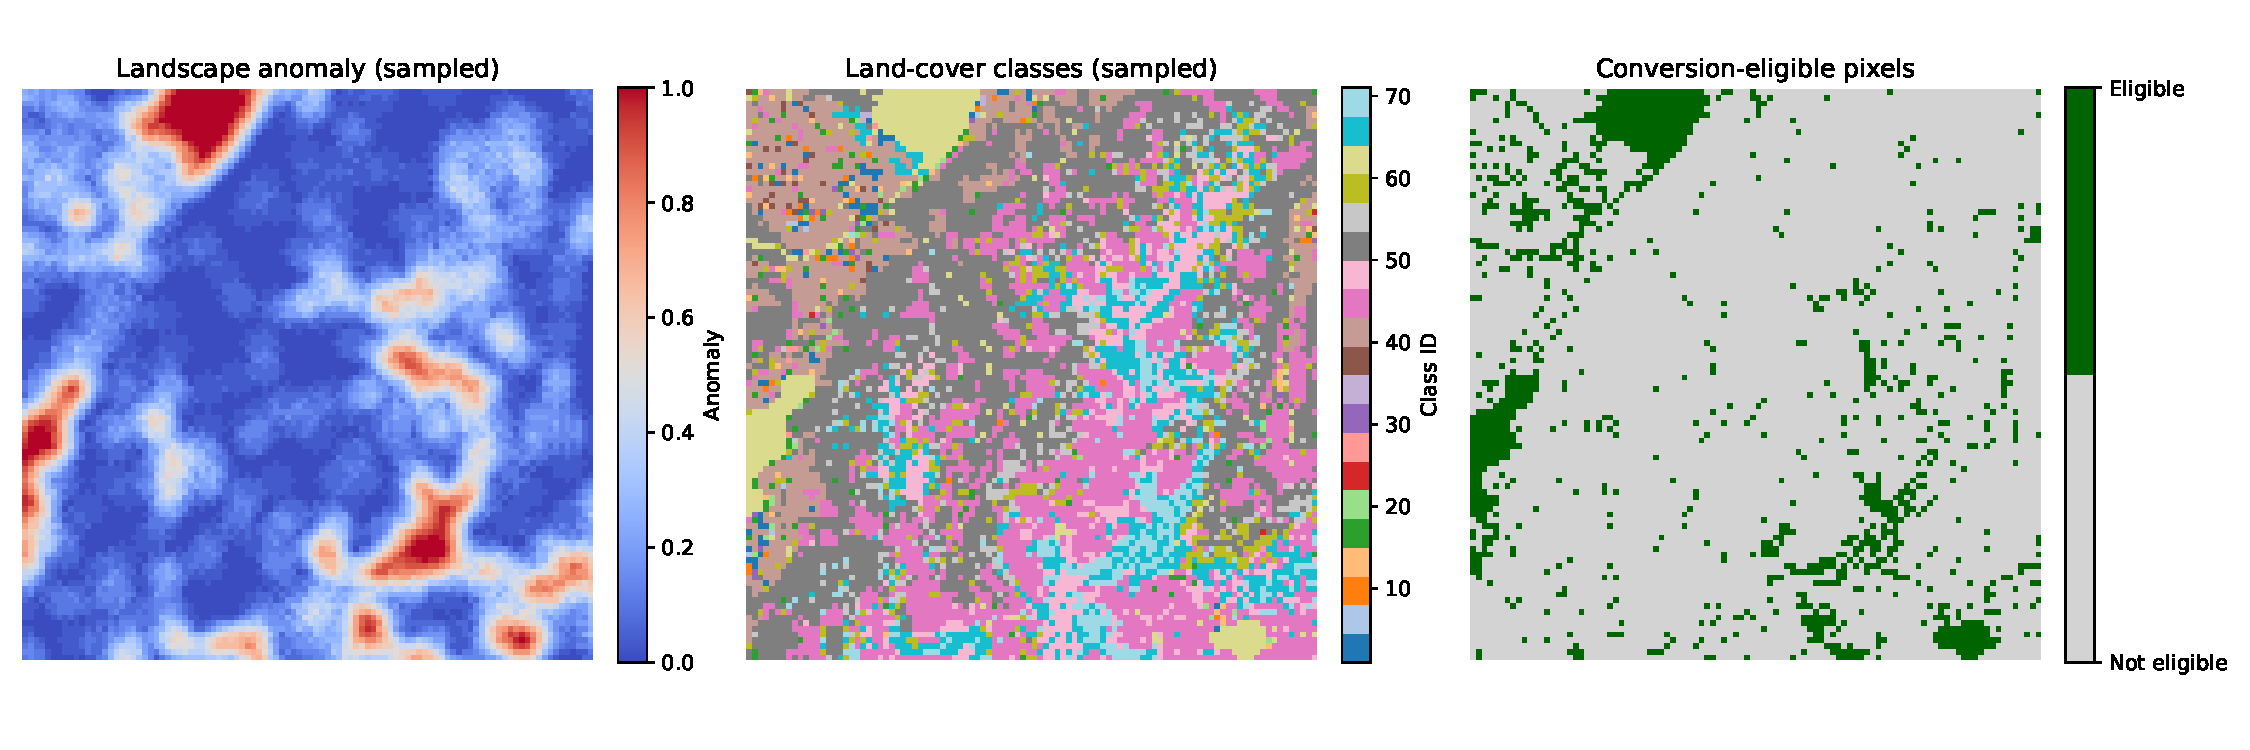
\includegraphics[keepaspectratio]{optimization_results_analysis_files/figure-pdf/landscape-sensitivity-test-1.pdf}}

Different intensities of conversion produce only small changes to
objective value/

\pandocbounded{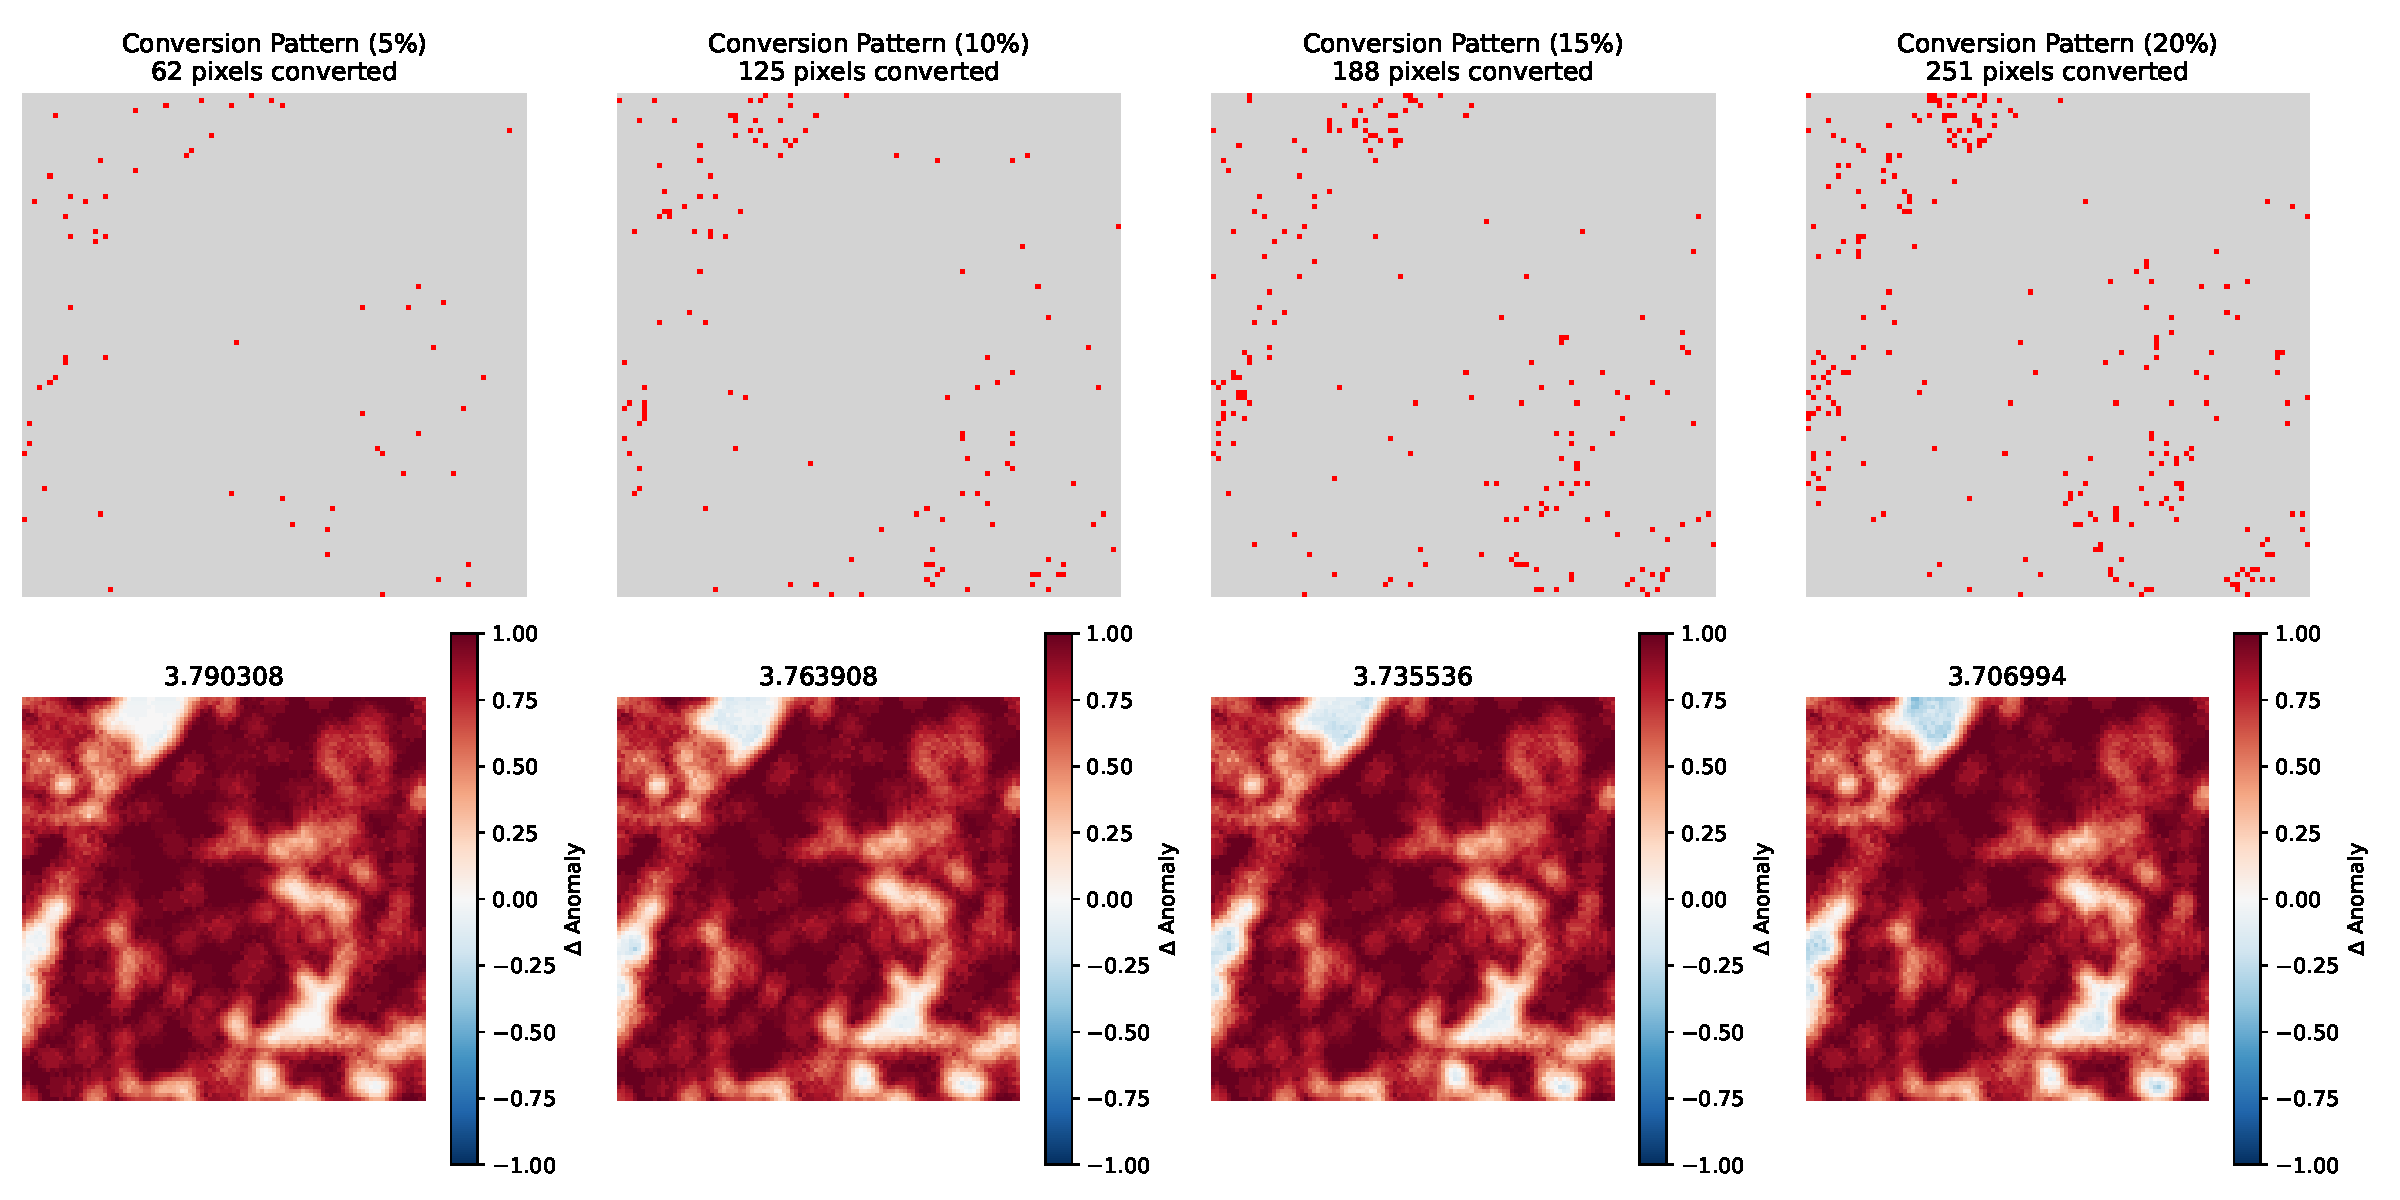
\includegraphics[keepaspectratio]{optimization_results_analysis_files/figure-pdf/unnamed-chunk-2-3.pdf}}

\pandocbounded{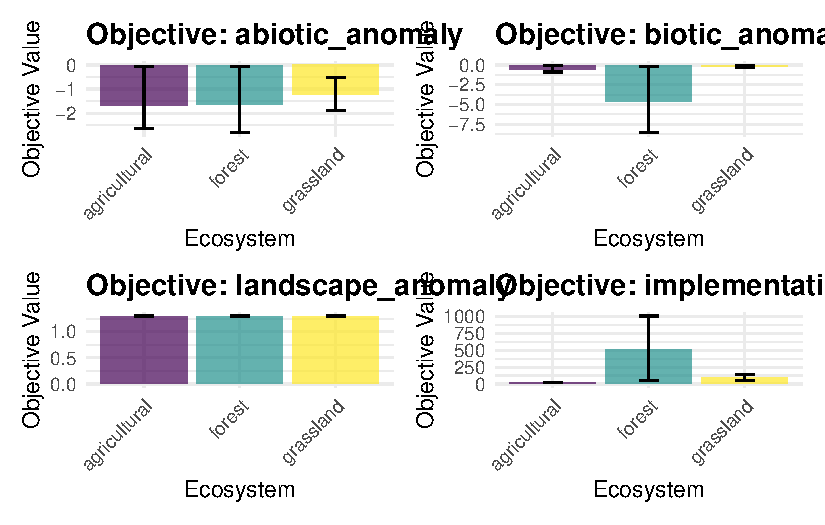
\includegraphics[keepaspectratio]{optimization_results_analysis_files/figure-pdf/ecosystem-objective-plots-5.pdf}}

\pandocbounded{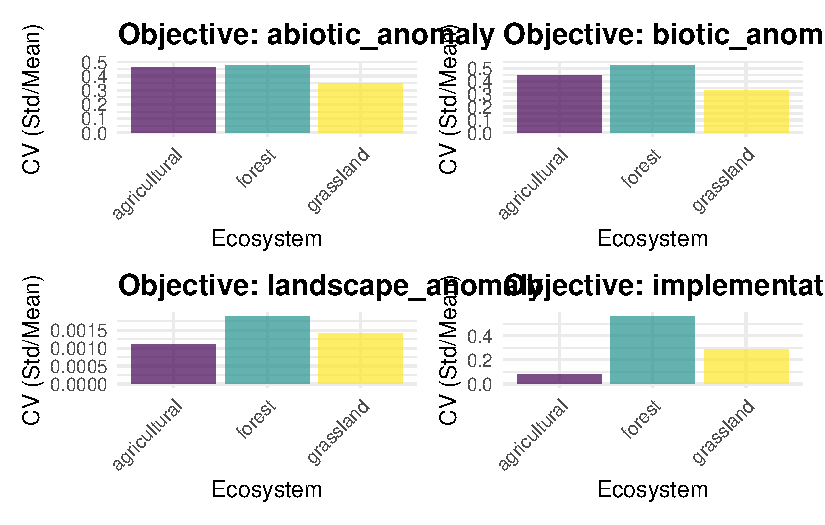
\includegraphics[keepaspectratio]{optimization_results_analysis_files/figure-pdf/ecosystem-objective-plots-6.pdf}}

\subsubsection{Population vs Pareto Front
Variance}\label{population-vs-pareto-front-variance}

For run without landscape objective.

\pandocbounded{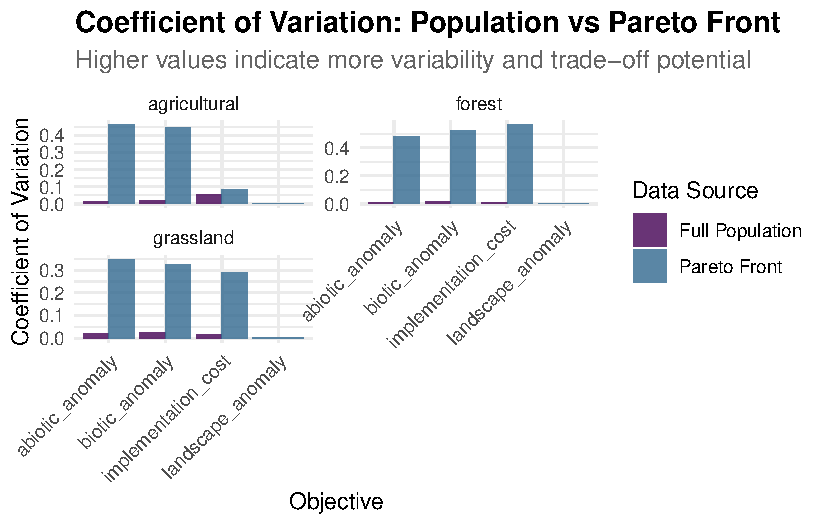
\includegraphics[keepaspectratio]{optimization_results_analysis_files/figure-pdf/combined-variance-analysis-1.pdf}}

\subsubsection{Evolution Tracking}\label{evolution-tracking}

Hyperparameter and objective evolution, for run without landscape
objective.

\pandocbounded{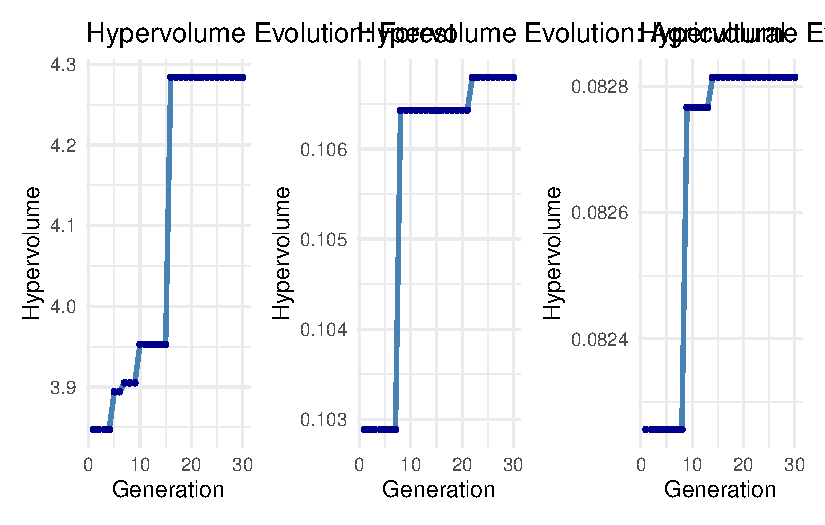
\includegraphics[keepaspectratio]{optimization_results_analysis_files/figure-pdf/ecosystem-evolution-analysis-1.pdf}}

\pandocbounded{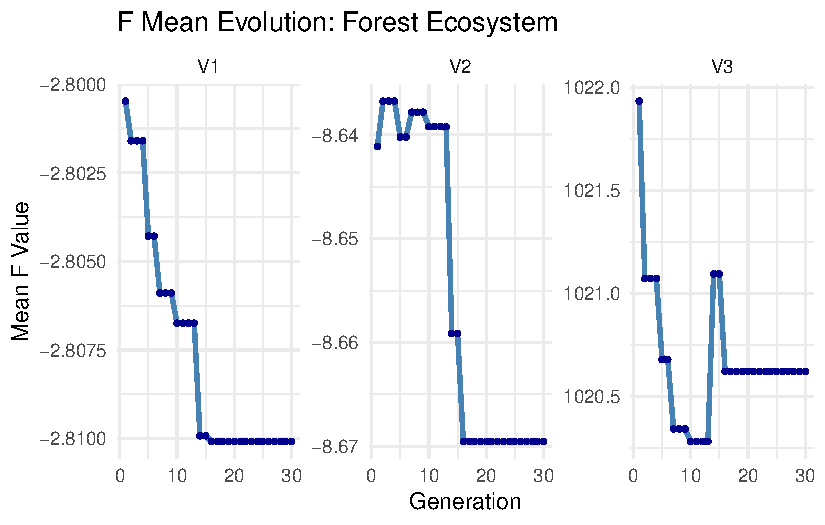
\includegraphics[keepaspectratio]{optimization_results_analysis_files/figure-pdf/ecosystem-evolution-analysis-2.pdf}}

\pandocbounded{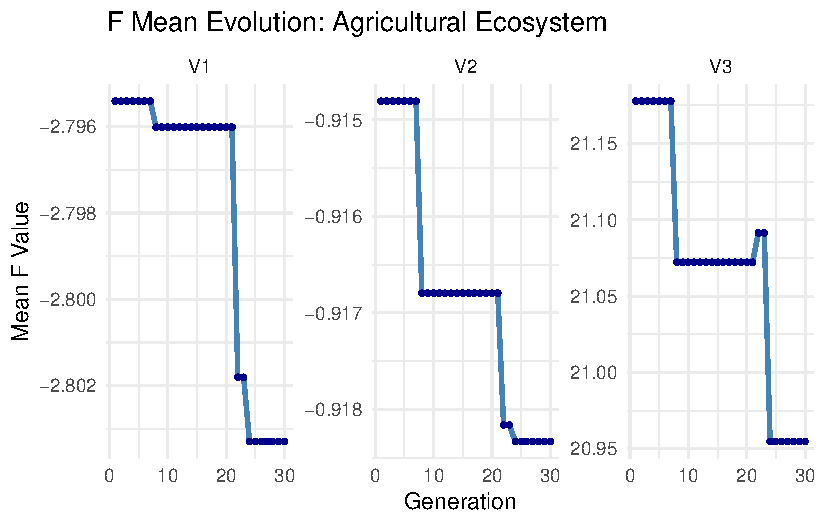
\includegraphics[keepaspectratio]{optimization_results_analysis_files/figure-pdf/ecosystem-evolution-analysis-3.pdf}}

\pandocbounded{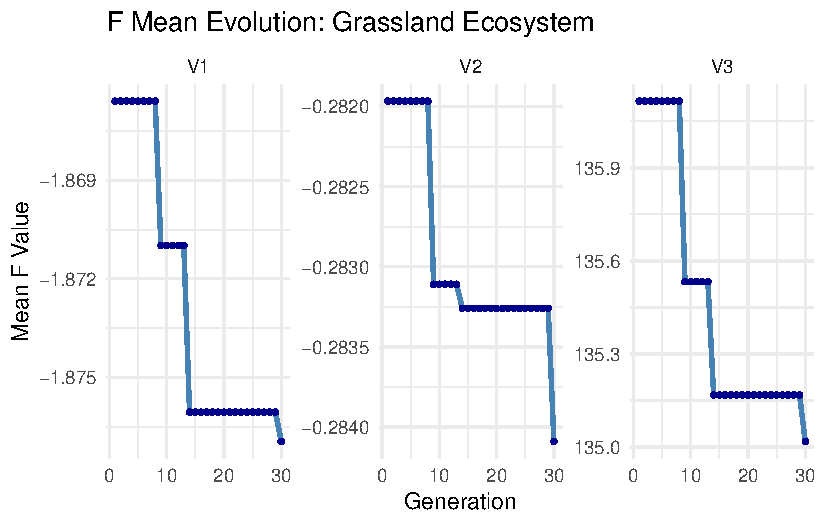
\includegraphics[keepaspectratio]{optimization_results_analysis_files/figure-pdf/ecosystem-evolution-analysis-4.pdf}}

\begin{center}\rule{0.5\linewidth}{0.5pt}\end{center}




\end{document}
